% Лабораторная работа по АСиСу № 1
% Михедов Константин Константинович

% Тип документа: статья, на бумаге А4
\documentclass[a4paper]{article}

% Подключение сторонних tex файлов 
\usepackage{import}


% Основные данные - ВУЗ, факультет, город...
\import{./../../stuff/tex}{config.tex}

% Подключение необходимых зависимостей
\import{./../../stuff/tex/settings}{packages.tex}
% Настройка подключенных пакетов
\import{./../../stuff/tex/settings}{preferences.tex}


% Шаблон титульной страницы 
\import{./../../stuff/tex/templates}{title.tex}
% Упрощенный блок "выполнил"
\import{./../../stuff/tex/templates}{sign1.tex}
% Макрос для содержания
\import{./../../stuff/tex/templates}{toc.tex}

% Определяем название документа
\title{
  Лабораторная работа №1 по курсу \\
  <<Проектный семинар>>  
}
% Отключаем отображение правительства
\renewcommand{\government}{}
% Отключаем сокращенное нзавание университета
\renewcommand{\subuniversity}{}
% Указываем преподавателя
\renewcommand{\shortteachername}{Минченков В.О.}


% Путь до внешних изображений
\graphicspath{ {./figures/}}


% Основной текст работы
\begin{document}
  \templatedtitlepage
  
  \toc
  \section{Ход работы}

  \subsection{Часть 1}

  Для работы необходимо создать виртуальную машину. Так как для использования
  был предложен готовый образ - воспользуемся им.
  \begin{figure}[H]
    \centering
    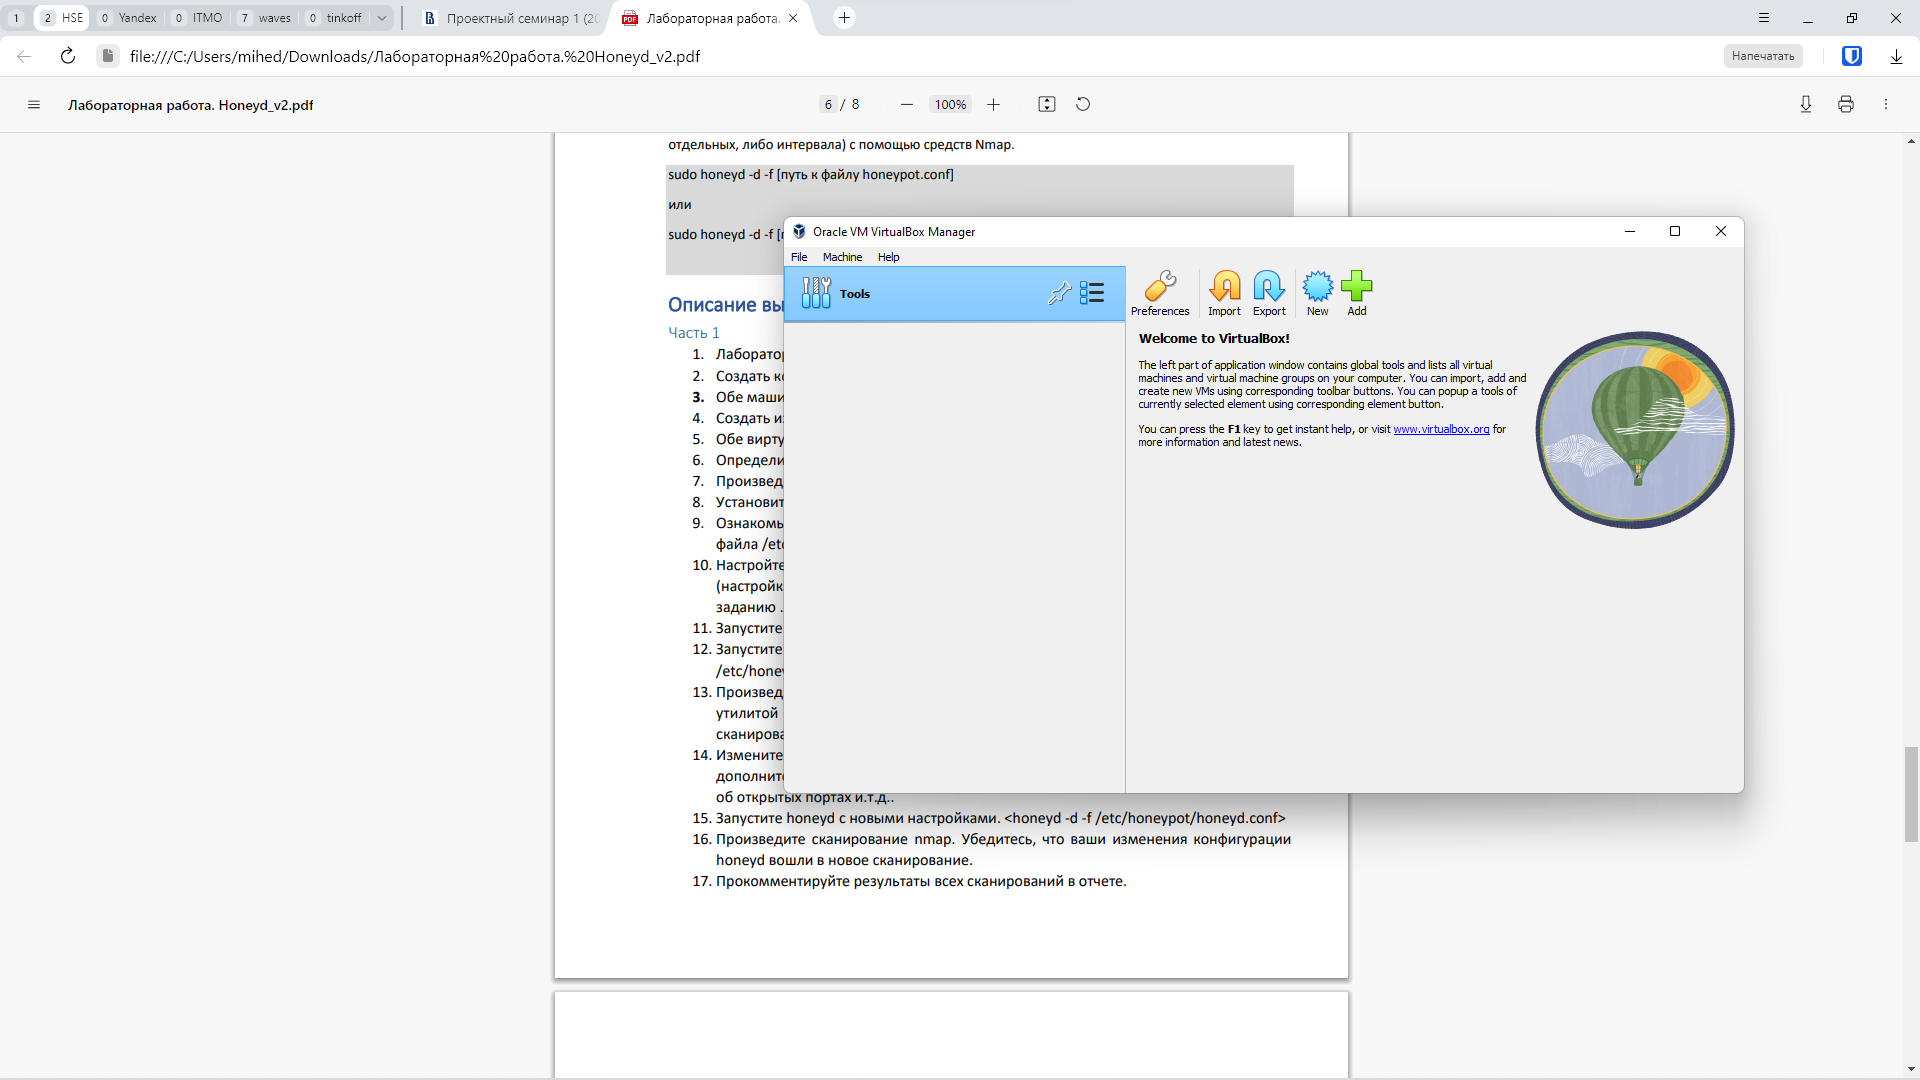
\includegraphics[width=0.85\textwidth]{00_00 (2)}
    \caption{Запускаем импорт образа системы}
  \end{figure}

  \begin{figure}[H]
    \centering
    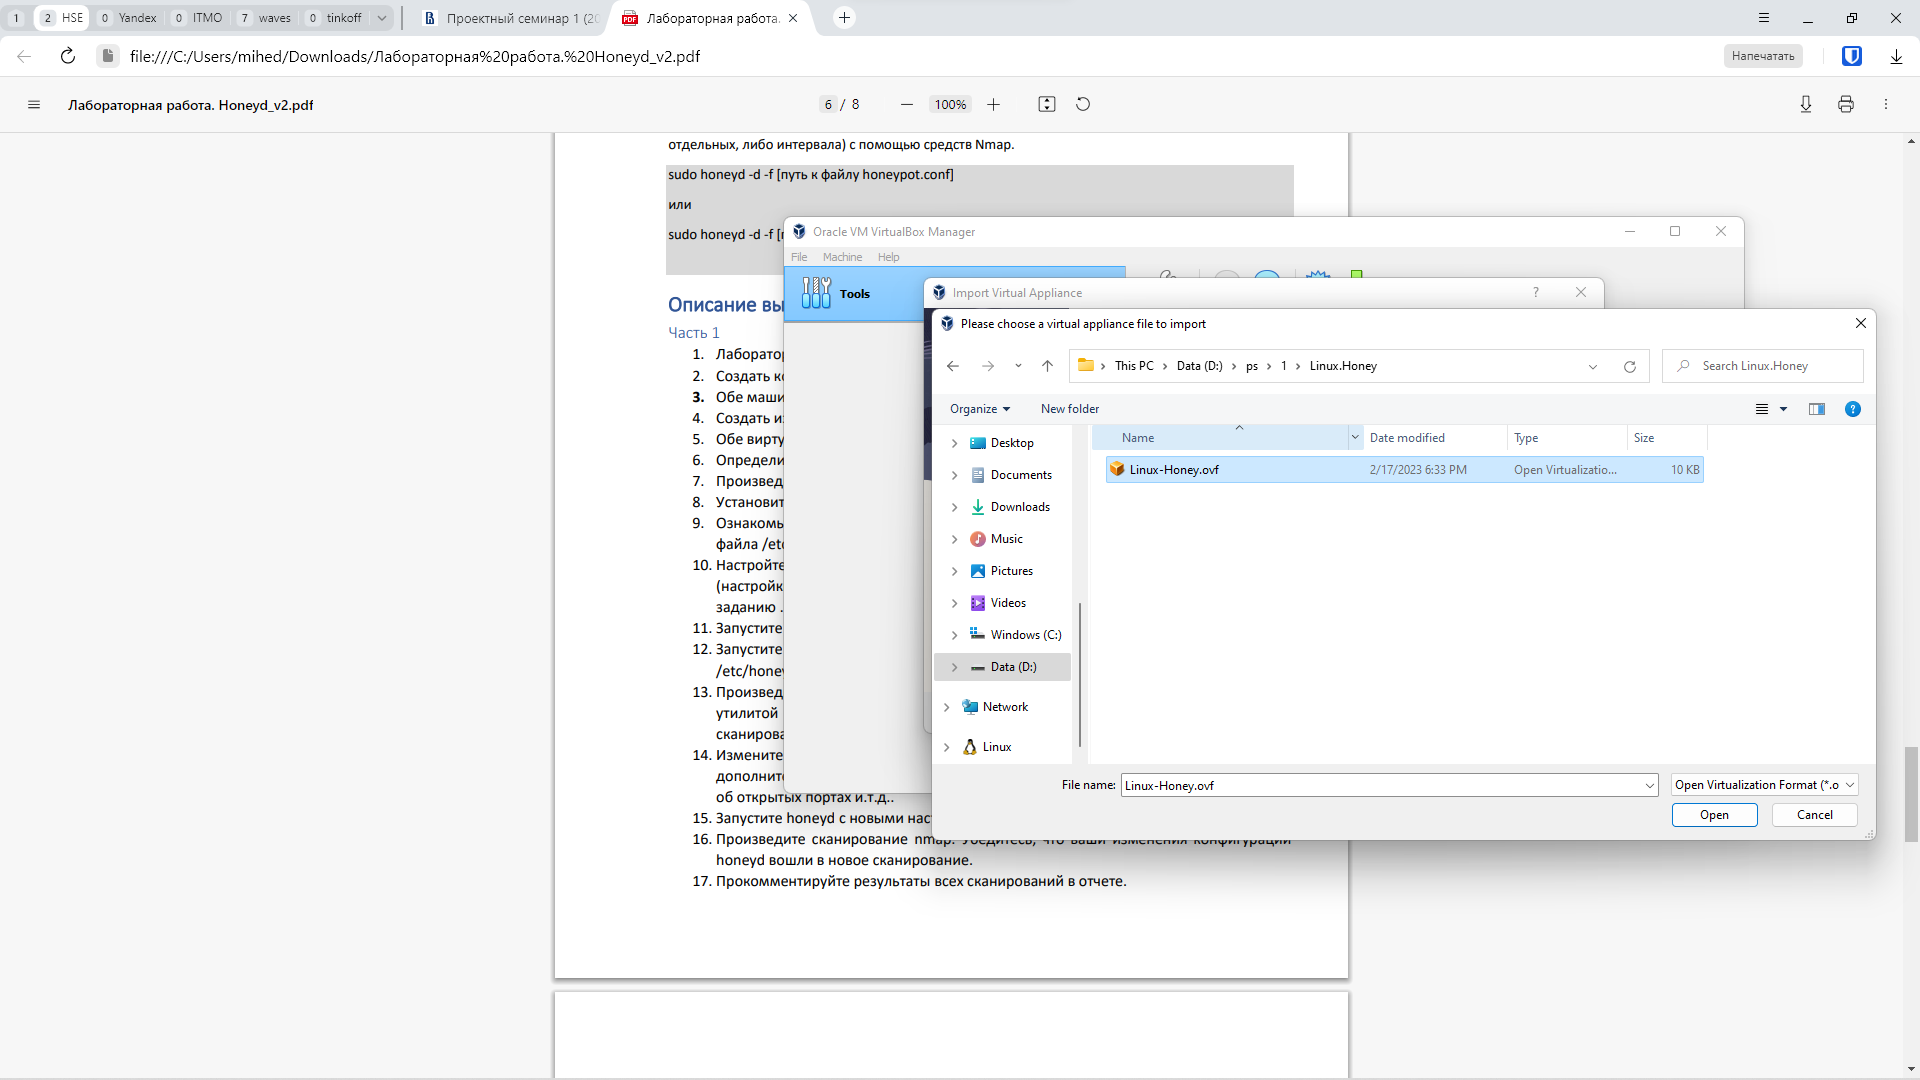
\includegraphics[width=0.85\textwidth]{00_00 (4)}
    \caption{Выбираем необходимый образ}
  \end{figure}
  
  Данную машину будем использовать как основной сервер, то есть запустим на ней \textit{honeypot}.
  Также нужна машина, которая будет выполнять сканирование - \textit{attacker}. 
  Создадим его при помощи клонирования ранее созданного образа:
  
  \begin{figure}[H]
    \centering
    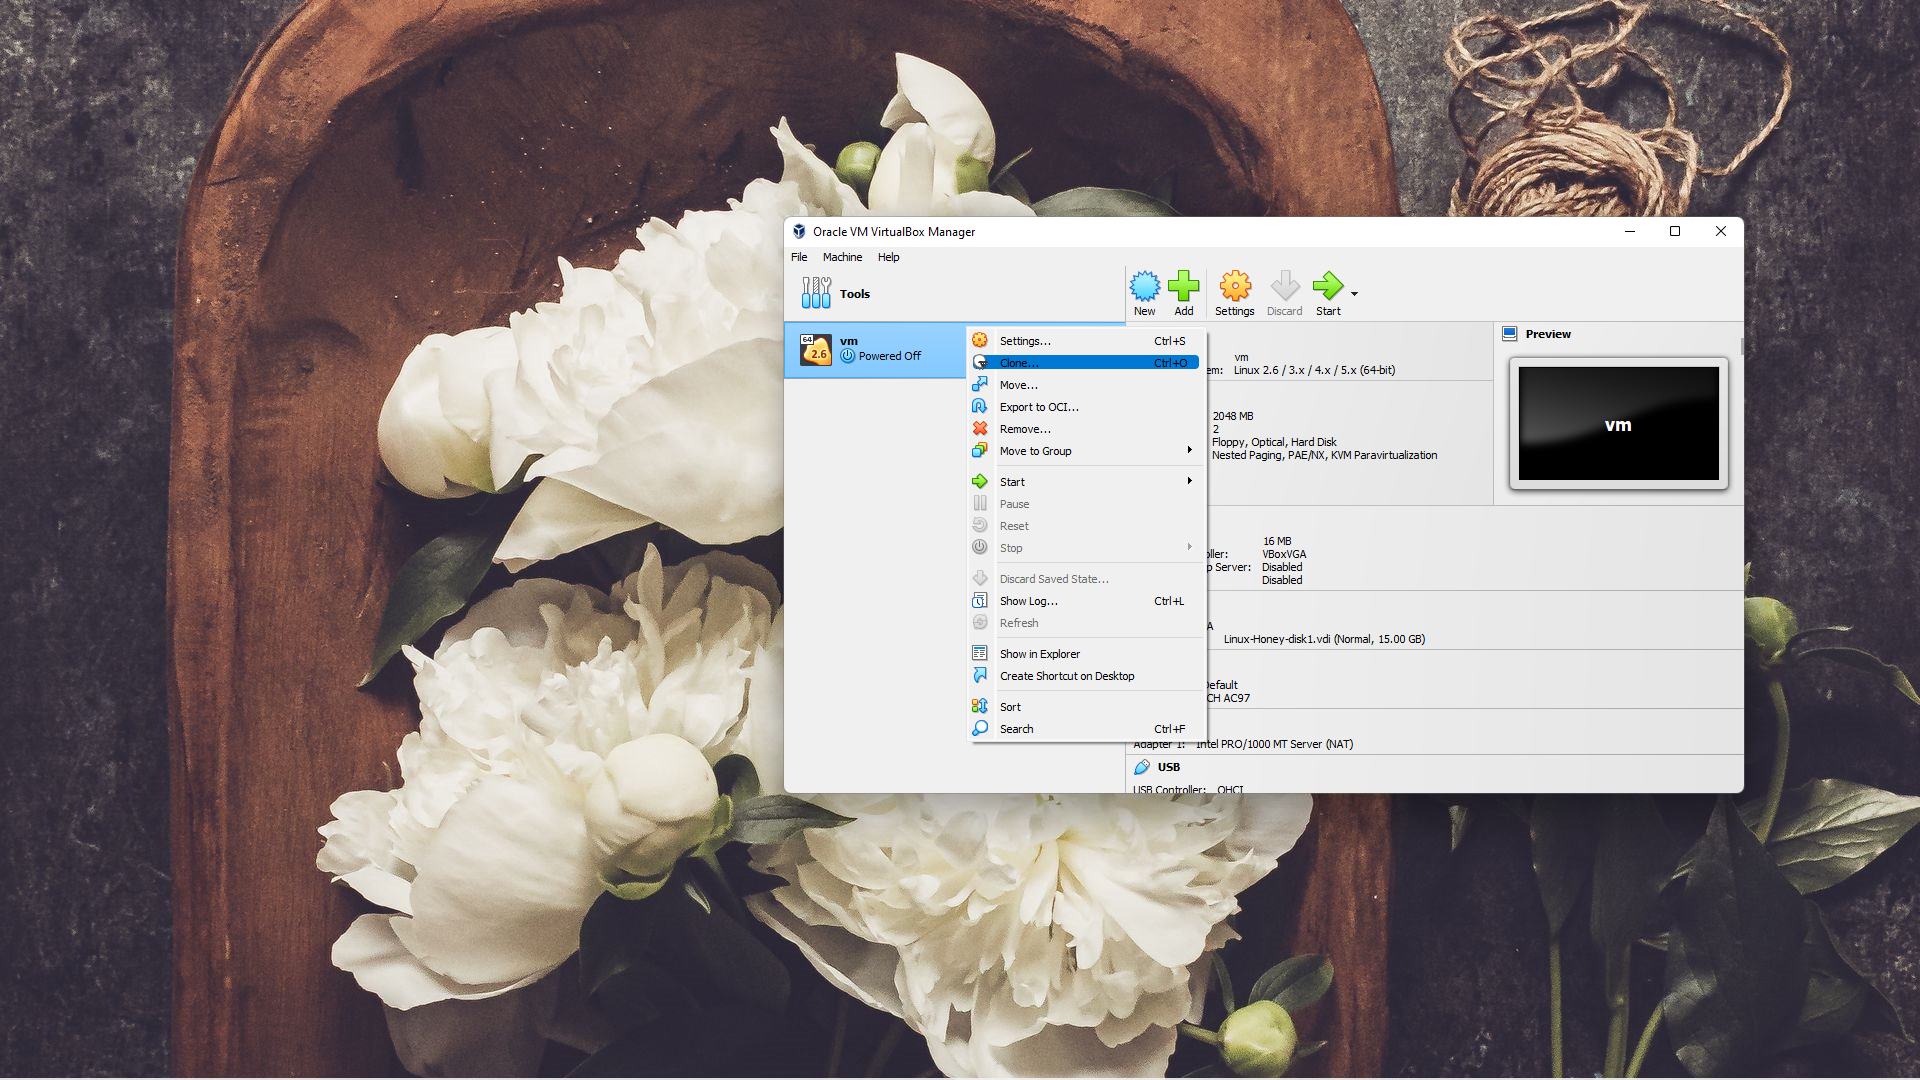
\includegraphics[width=0.85\textwidth]{01_00 (1)}
    \caption{Начинаем клонирование образа}
  \end{figure}
  
  \begin{figure}[H]
    \centering
    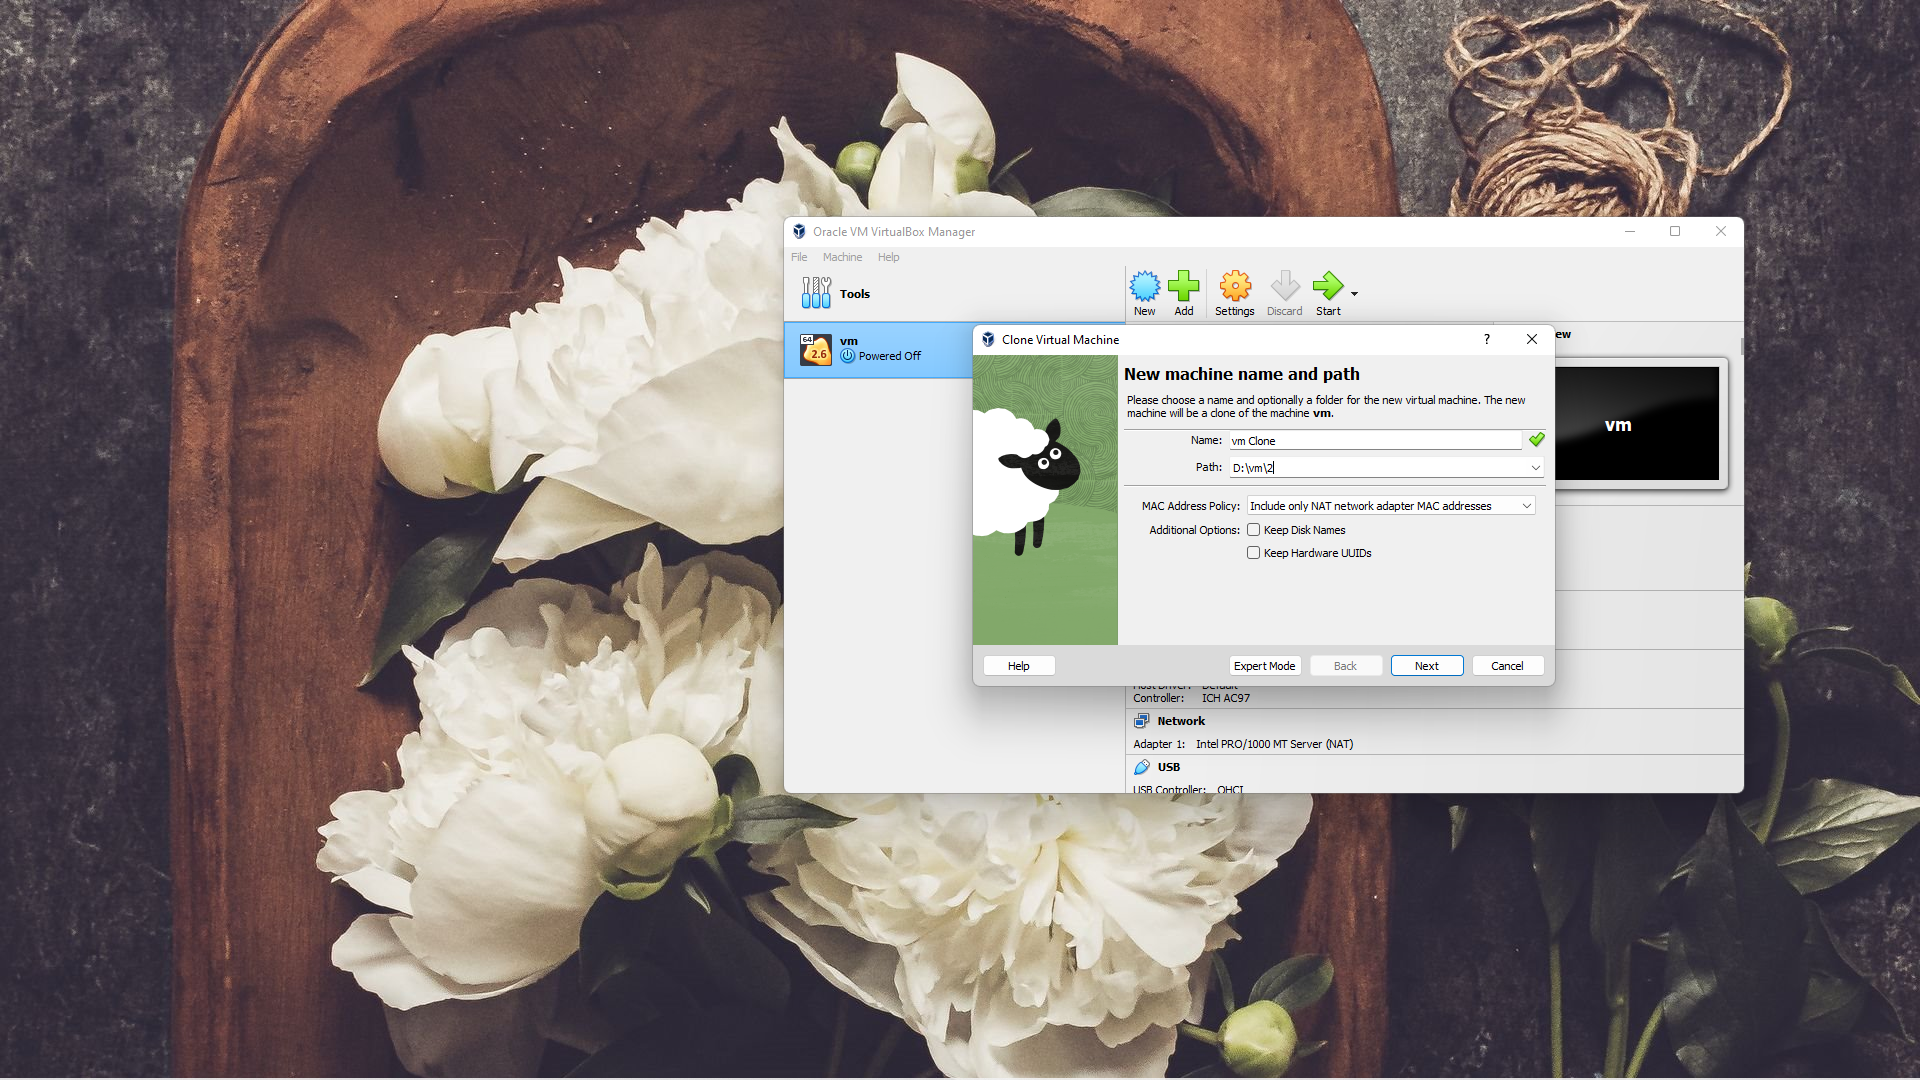
\includegraphics[width=0.85\textwidth]{01_00 (2)}
    \caption{Завершаем клонирование образа}
  \end{figure}

  \begin{figure}[H]
    \centering
    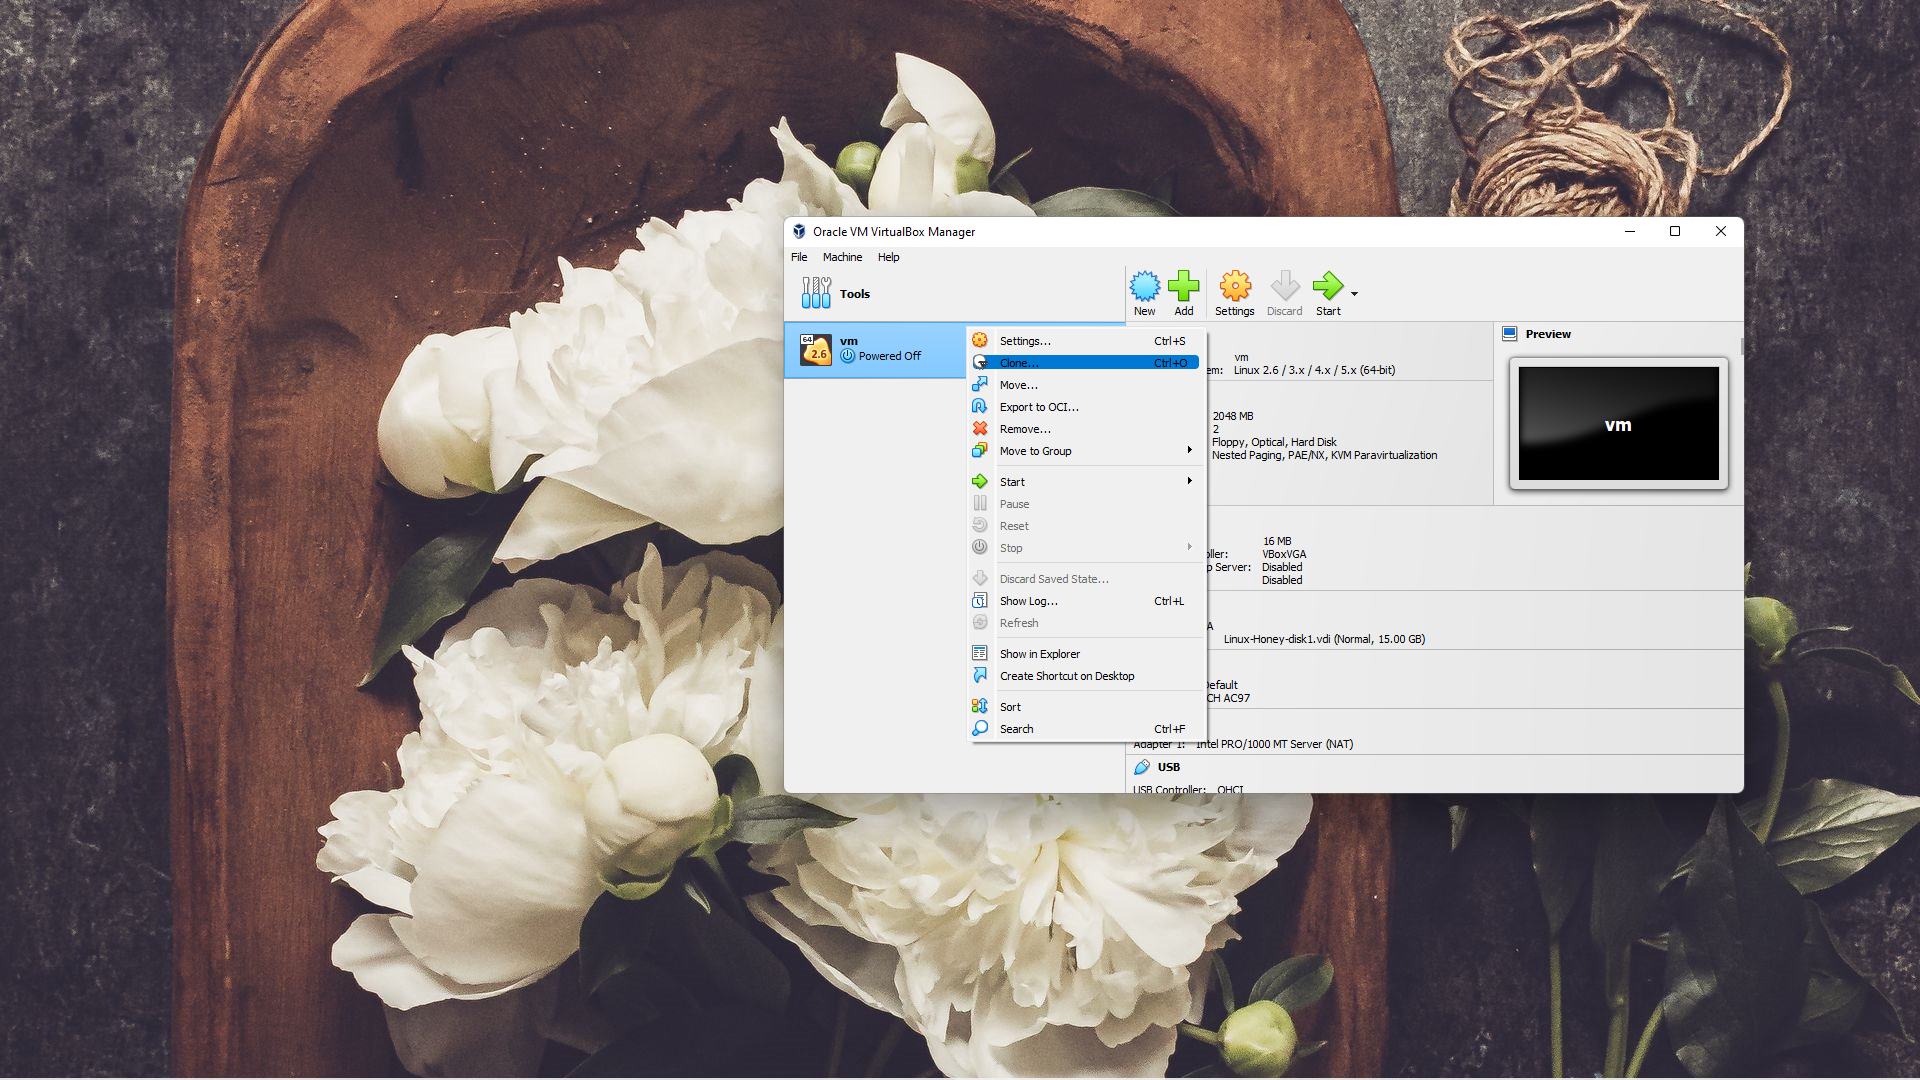
\includegraphics[width=0.85\textwidth]{01_00 (1)}
    \caption{Начинаем клонирование образа}
  \end{figure}

  Каждую из созданных виртуальных машин необходимо подключить к одной \textit{NAT}
  сети, чтобы появилась возможность их взаимодействия:

  \begin{figure}[H]
    \centering
    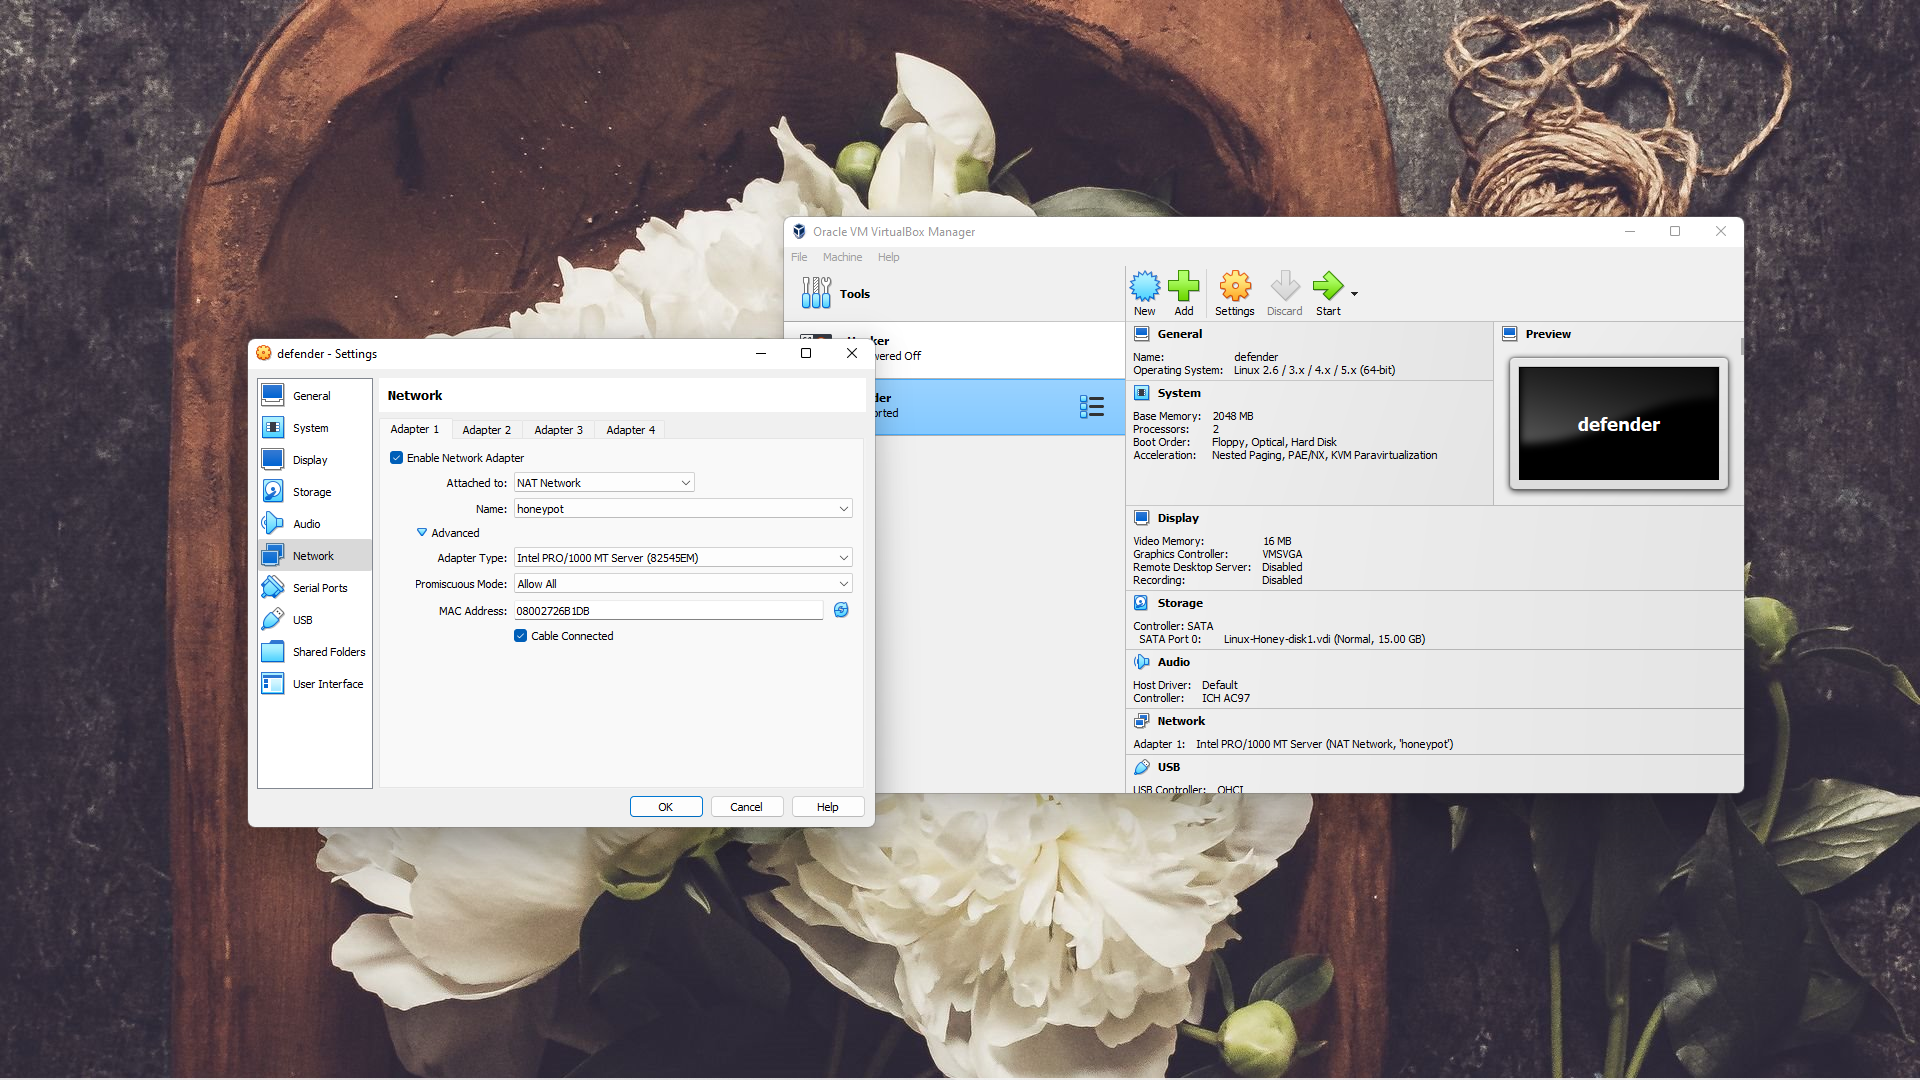
\includegraphics[width=0.85\textwidth]{01_00 (20)}
    \caption{Указываем настройки сетей}
  \end{figure}

  Теперь запускаем обе виртуальные машины и узнаем их \textit{IP} адреса
  при помощи команды \textit{ip a}

  \begin{figure}[H]
    \centering
    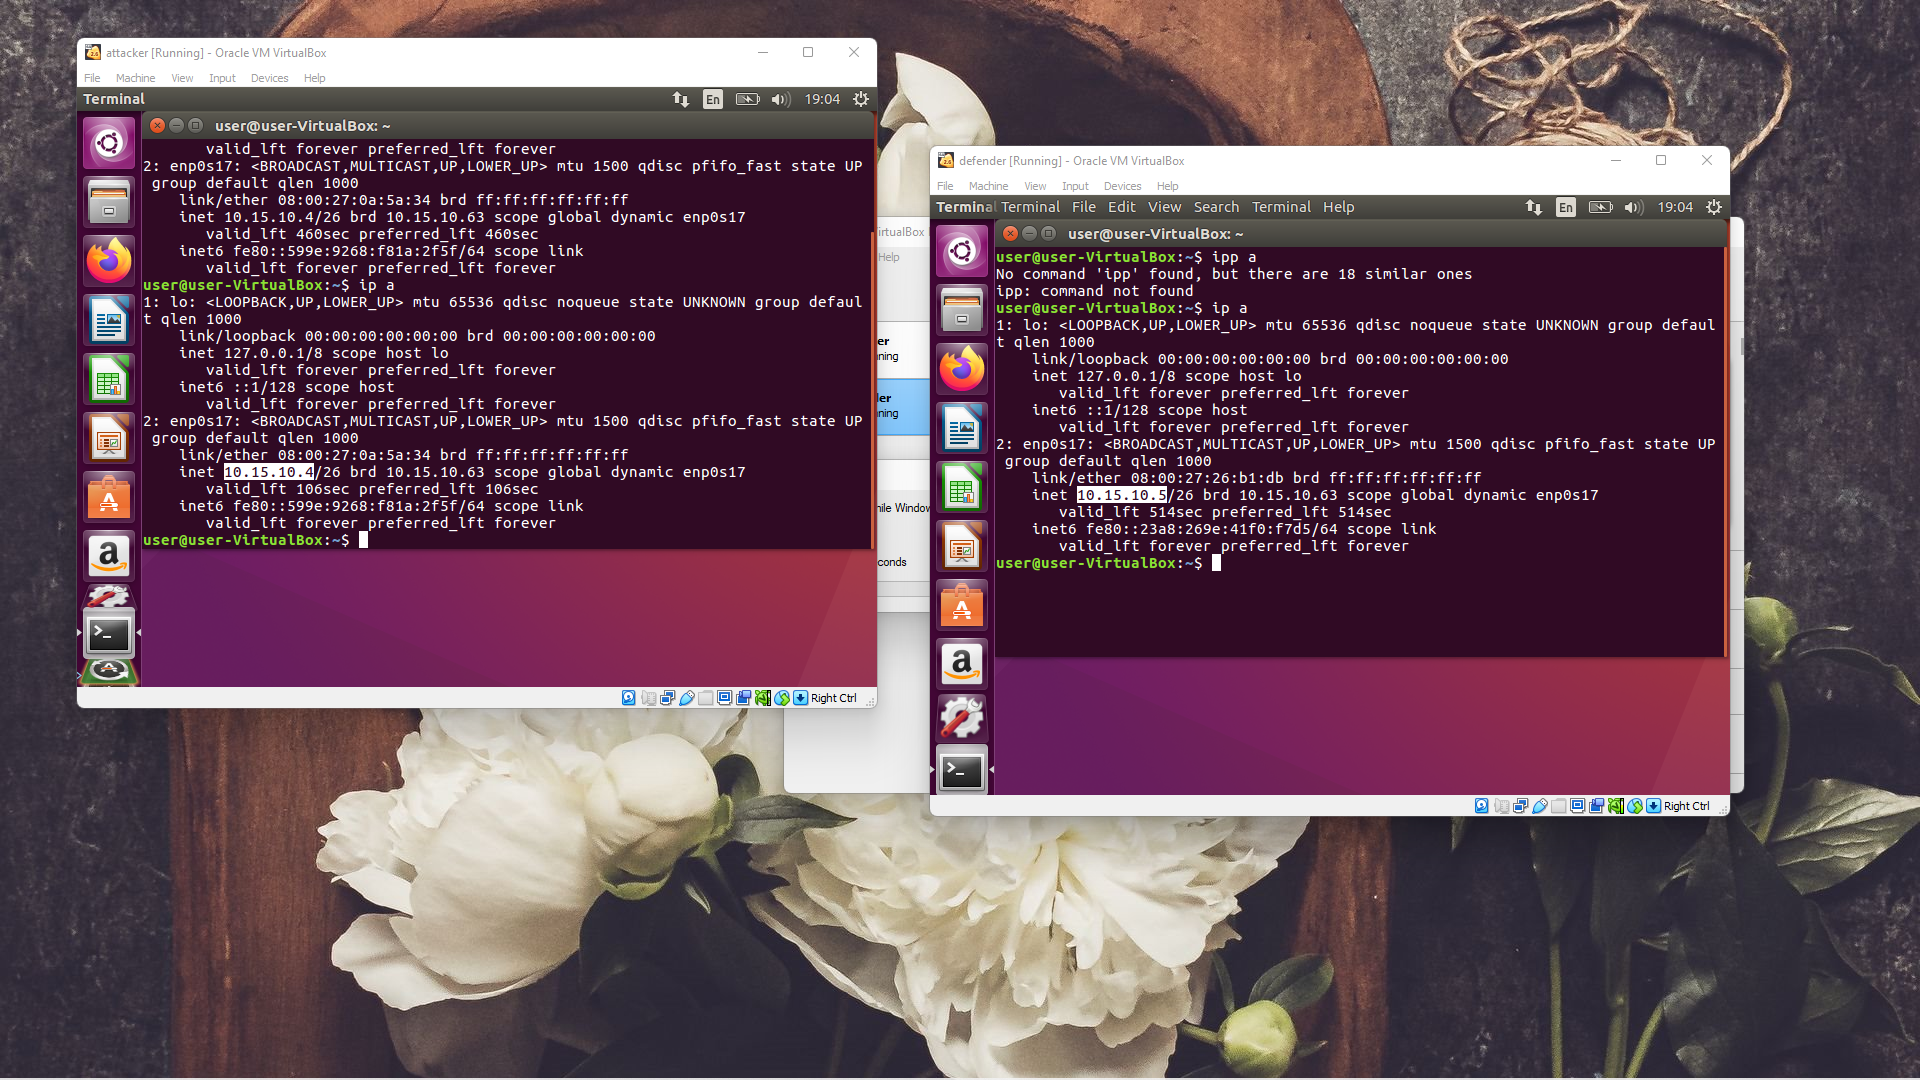
\includegraphics[width=0.85\textwidth]{01_00 (7)}
    \caption{Полученные IP адреса}
  \end{figure}

  Получается, что \textit{IPv4} основной хостовой машины, то есть той, на которой будет запущен \textit{honeypot},
  10.15.10.5, а адрес атакующей (сканирующей) машины - 10.15.10.4.

  Теперь необходимо обновить конфигурацию \textit{honeypot} с учетом найденных
  \textit{IP} адресов

  \begin{figure}[H]
    \centering
    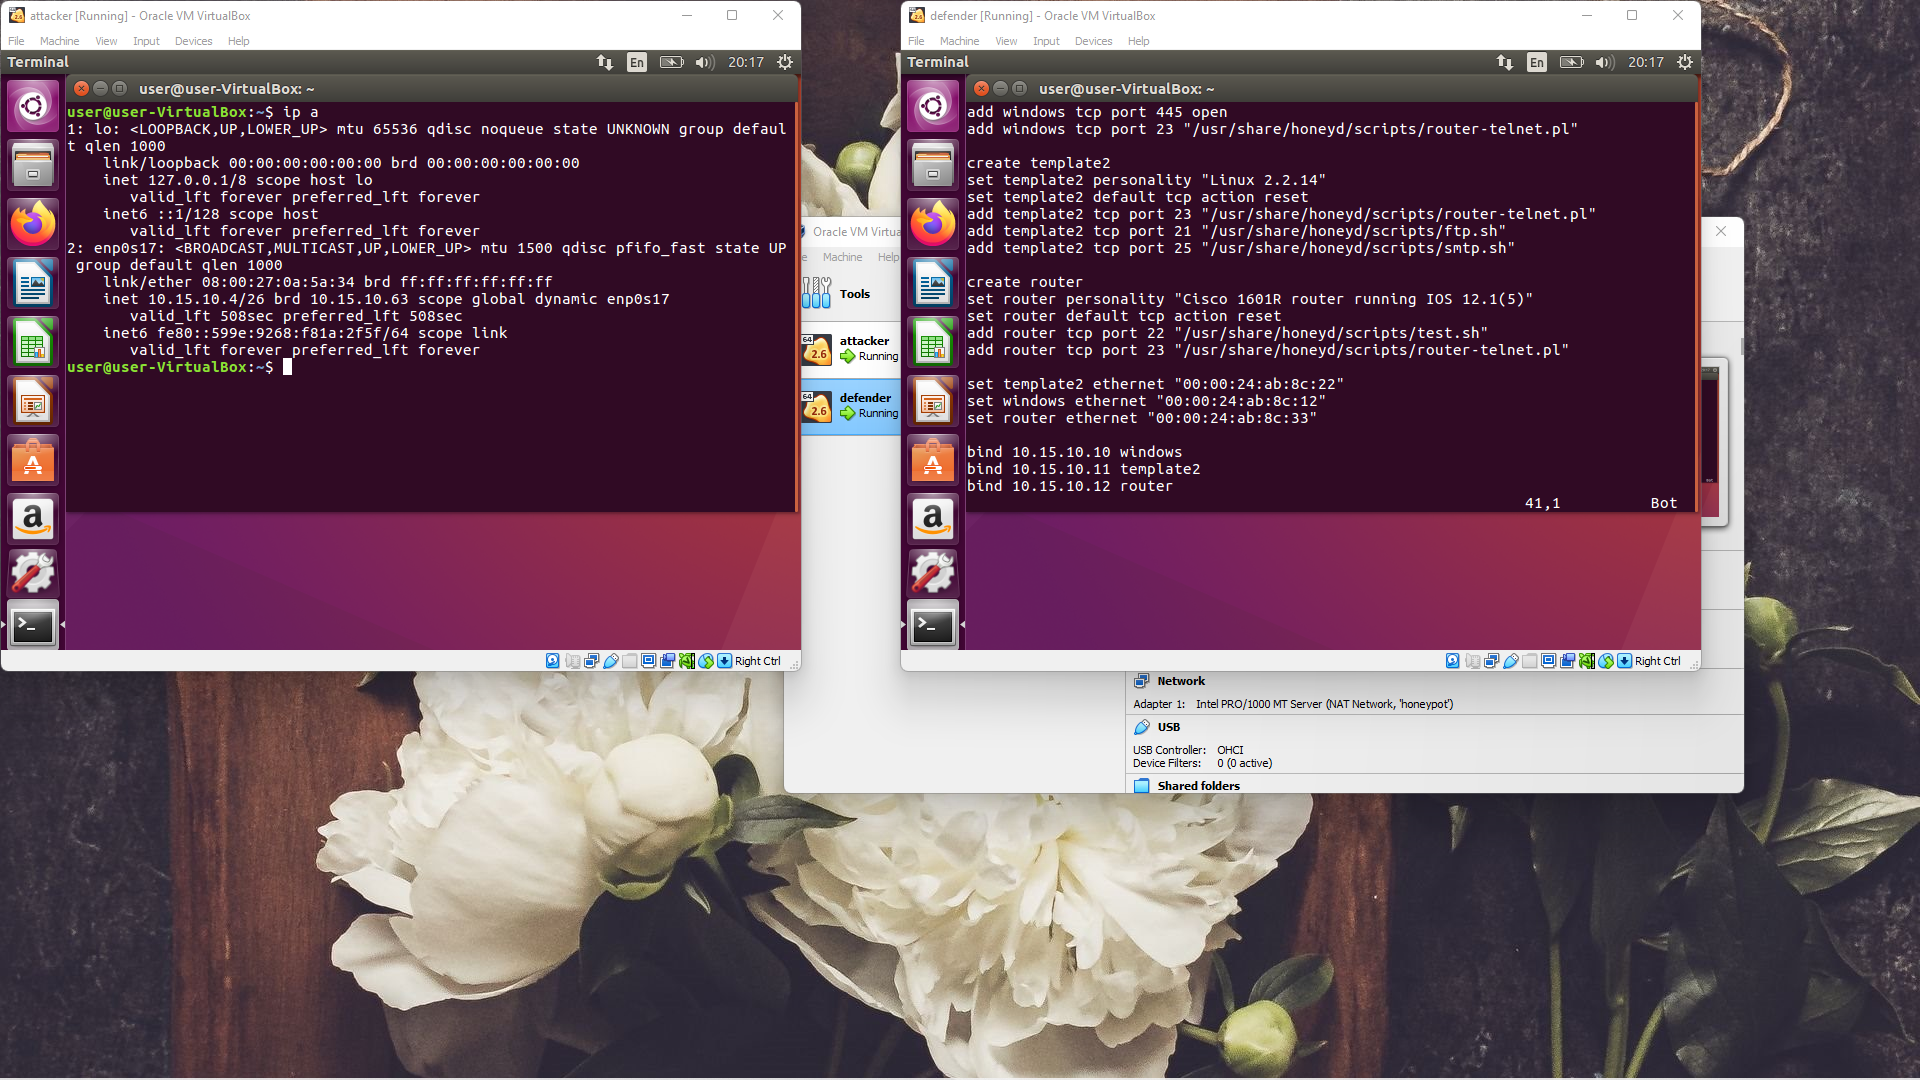
\includegraphics[width=0.85\textwidth]{01_00 (22)}
    \caption{Обновленная конфигурация}
  \end{figure}

  Далее можно запускать саму ловушку, а точнее сначала \textit{farpd},
  а затем уже сам \textit{honeypot}:
  
  \begin{figure}[H]
    \centering
    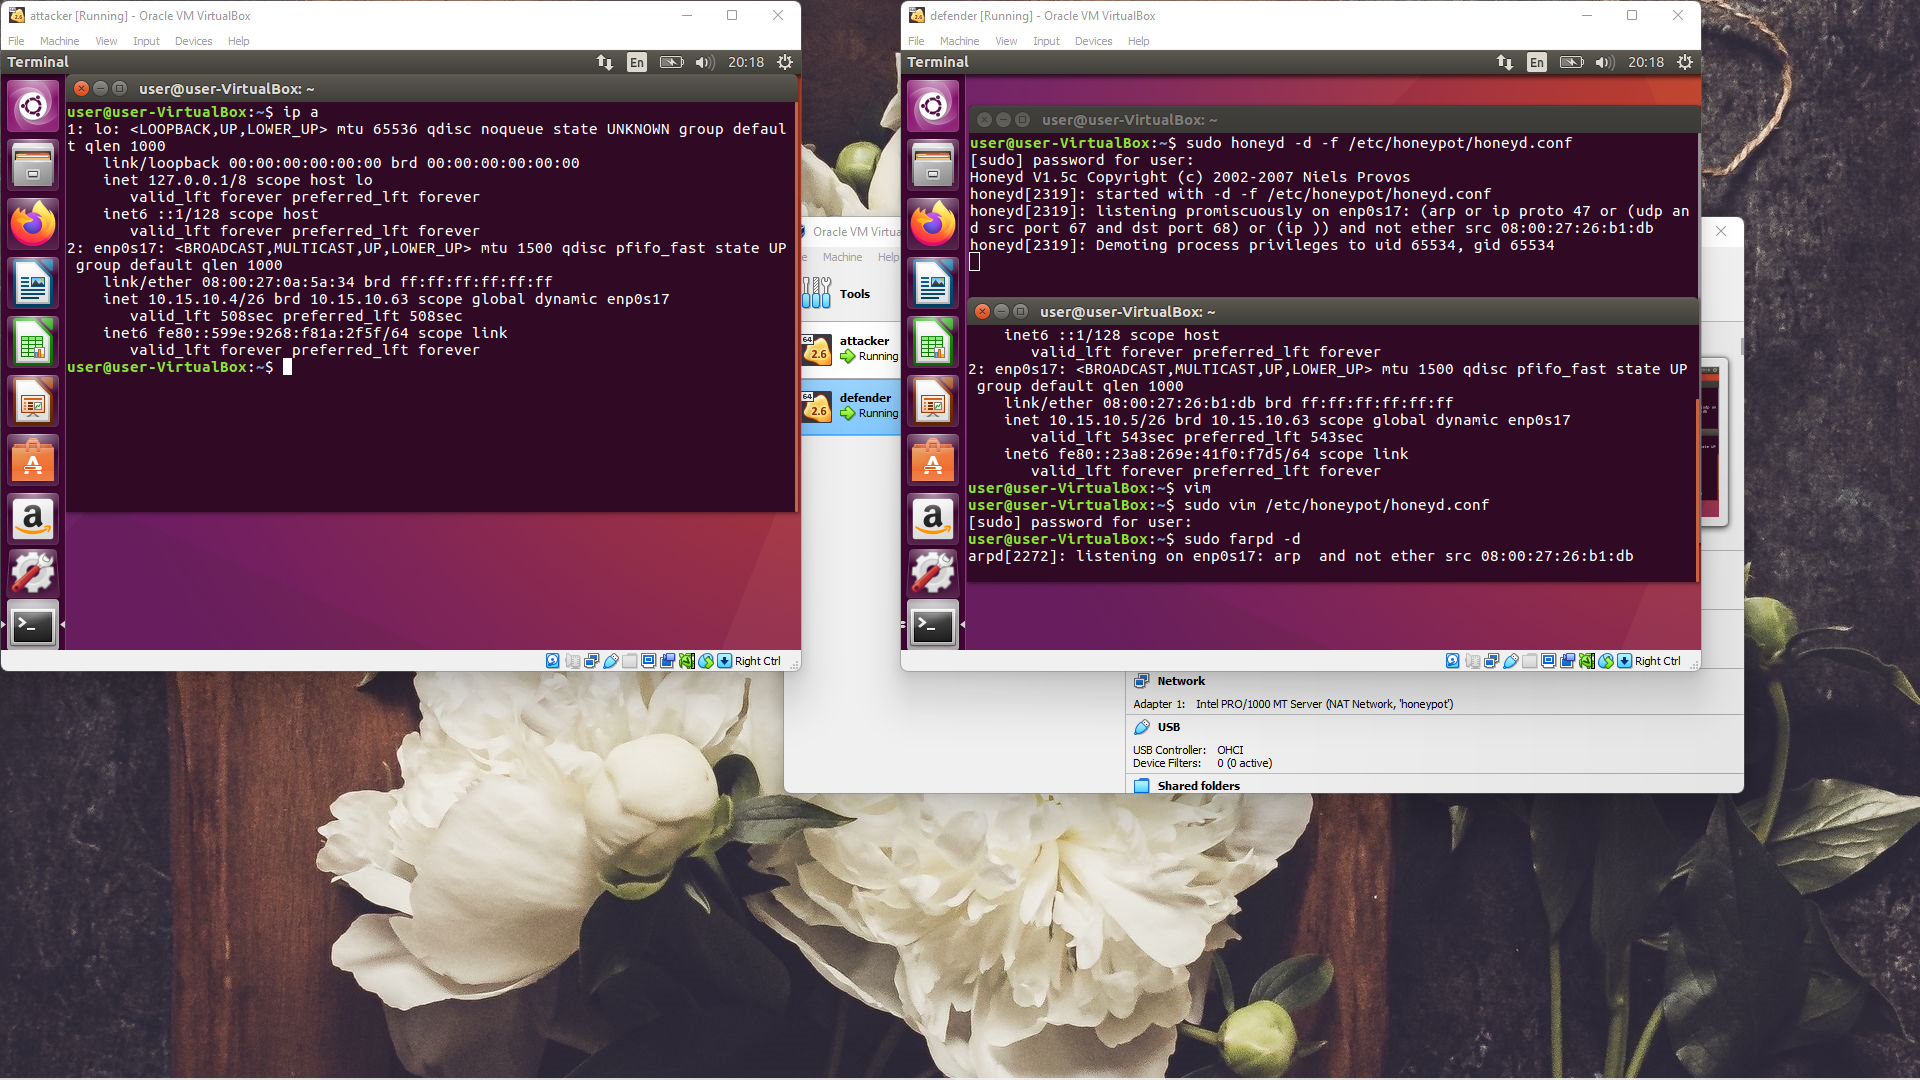
\includegraphics[width=0.85\textwidth]{01_00 (23)}
    \caption{Запущенная ловушка (справа)}
  \end{figure}

  Теперь можно производить различные виды сканирования и анализировать полученные результаты.

  \subsubsection{TCP connect}

  Чтобы просканировать сразу все необходимые \textit{IP} адреса, укажем их через пробел:

  \begin{figure}[H]
    \centering
    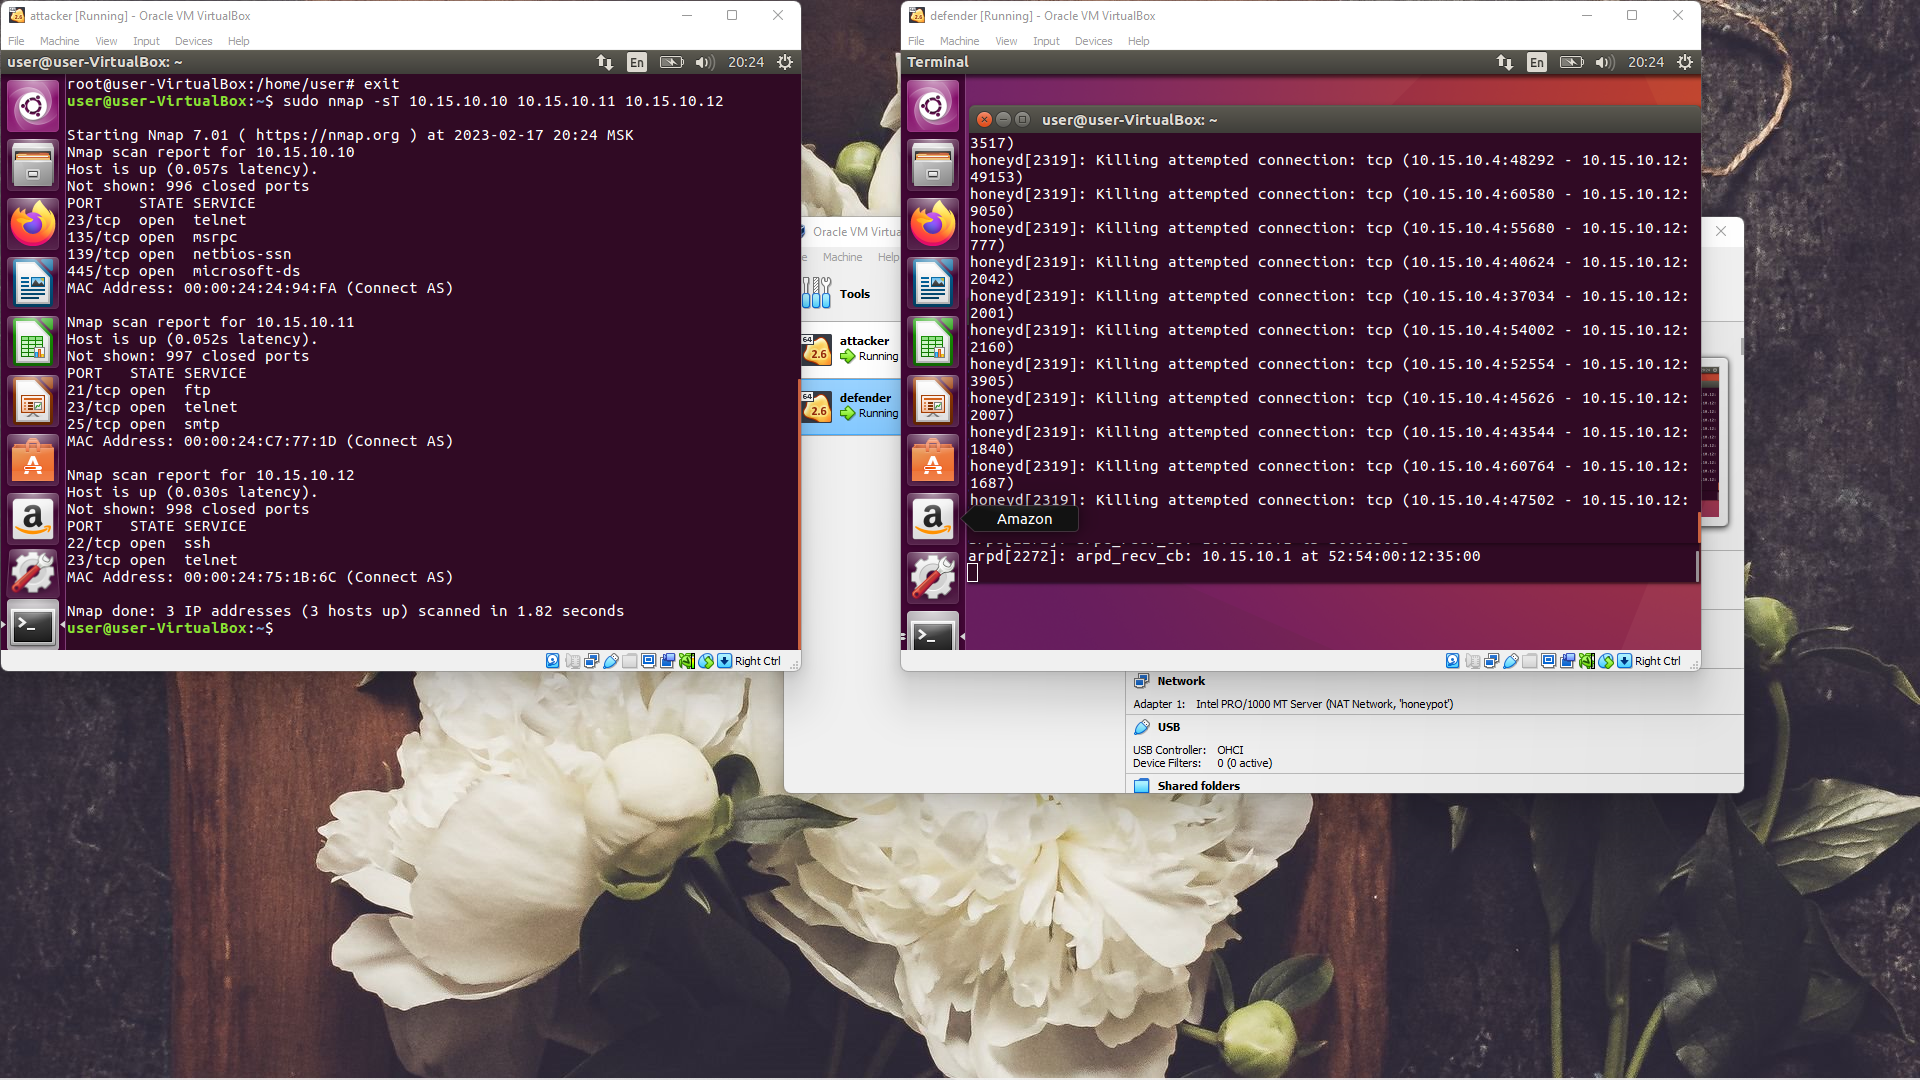
\includegraphics[width=0.85\textwidth]{01_00 (26)}
    \caption{TCP Connect сканирование}
  \end{figure}

  В данном случае результаты сканирования (список открытых портов) полностью
  совпадают с прописанным для \textit{honeypot} конфигом, следовательно
  данный вид сканирования работает абсолютно корректно.

  \subsubsection{TCP-SYN сканирование}

  \begin{figure}[H]
    \centering
    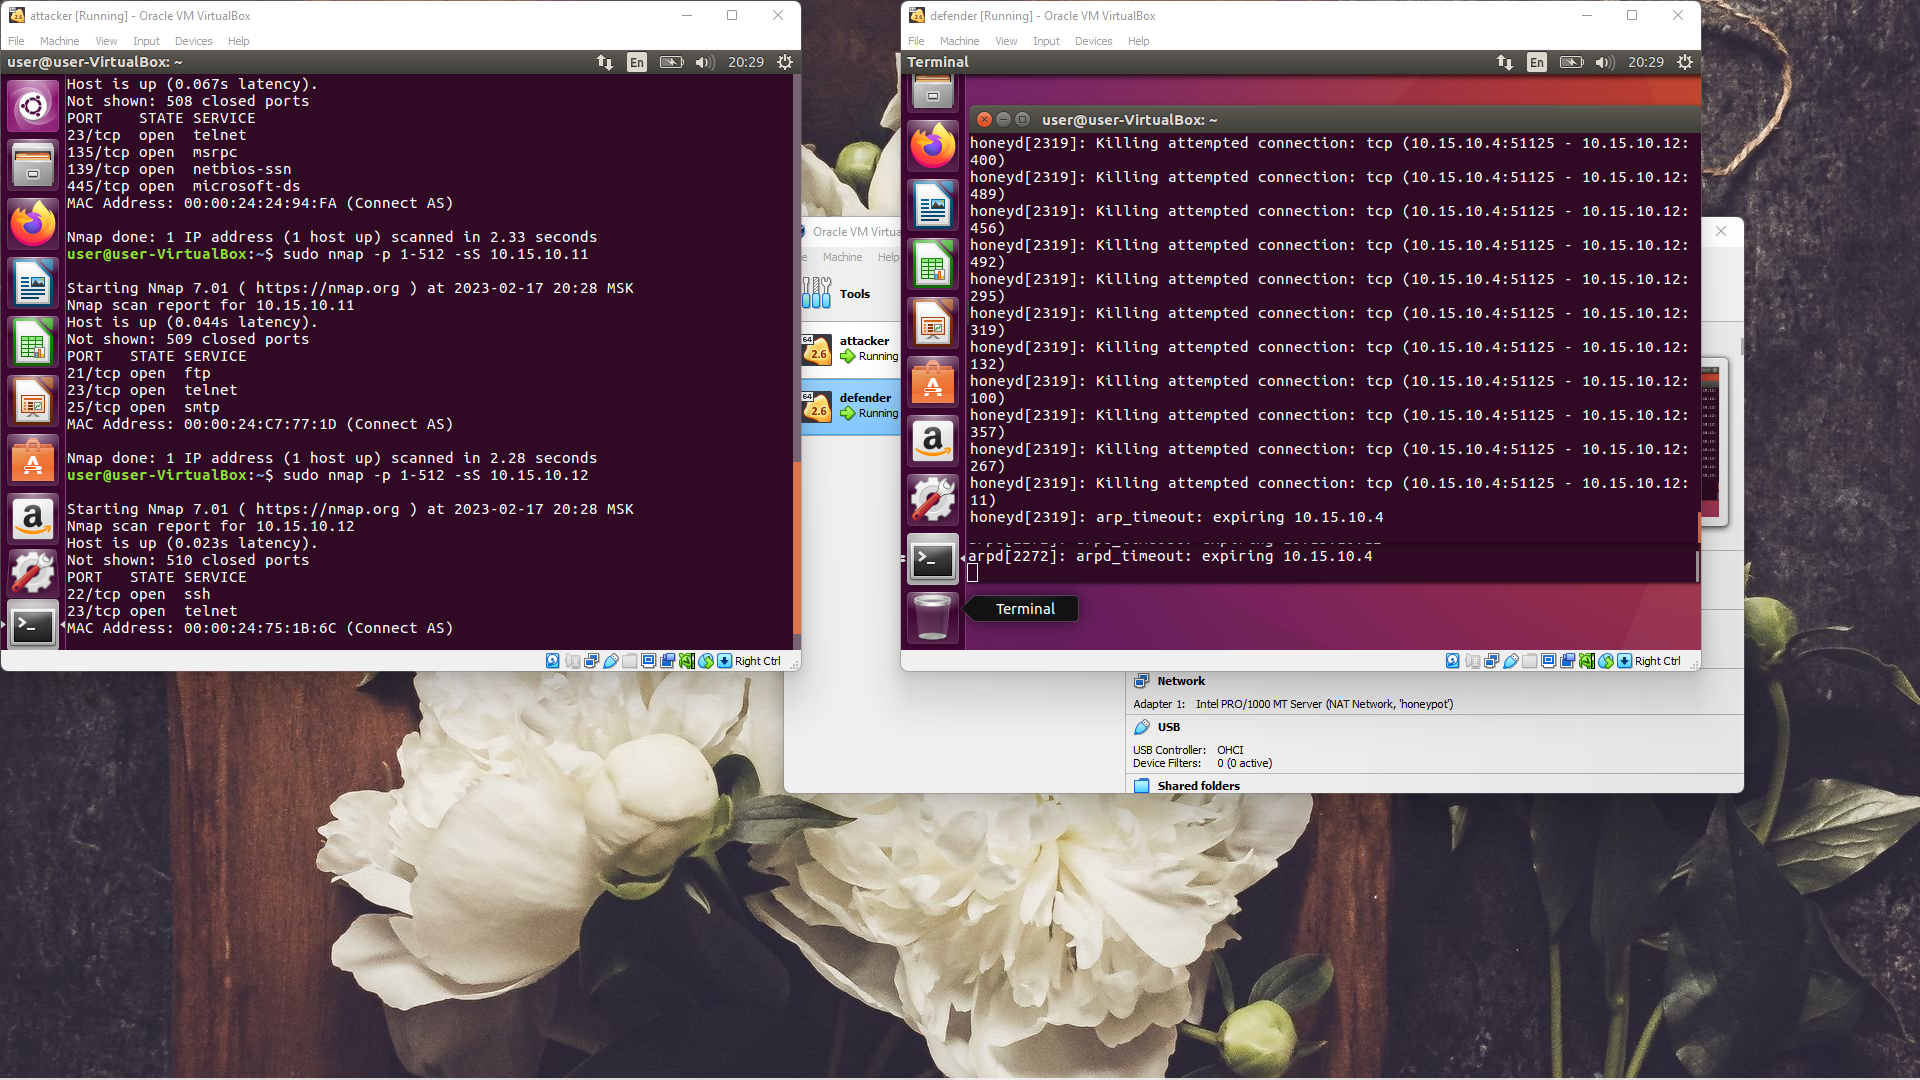
\includegraphics[width=0.85\textwidth]{01_00 (28)}
    \caption{TCP-SYN сканирование}
  \end{figure}

  Данный вид сканирования также хорошо показал себя на данной конфигурации.

  \subsubsection{Сканирование протоколов IP}

  \begin{figure}[H]
    \centering
    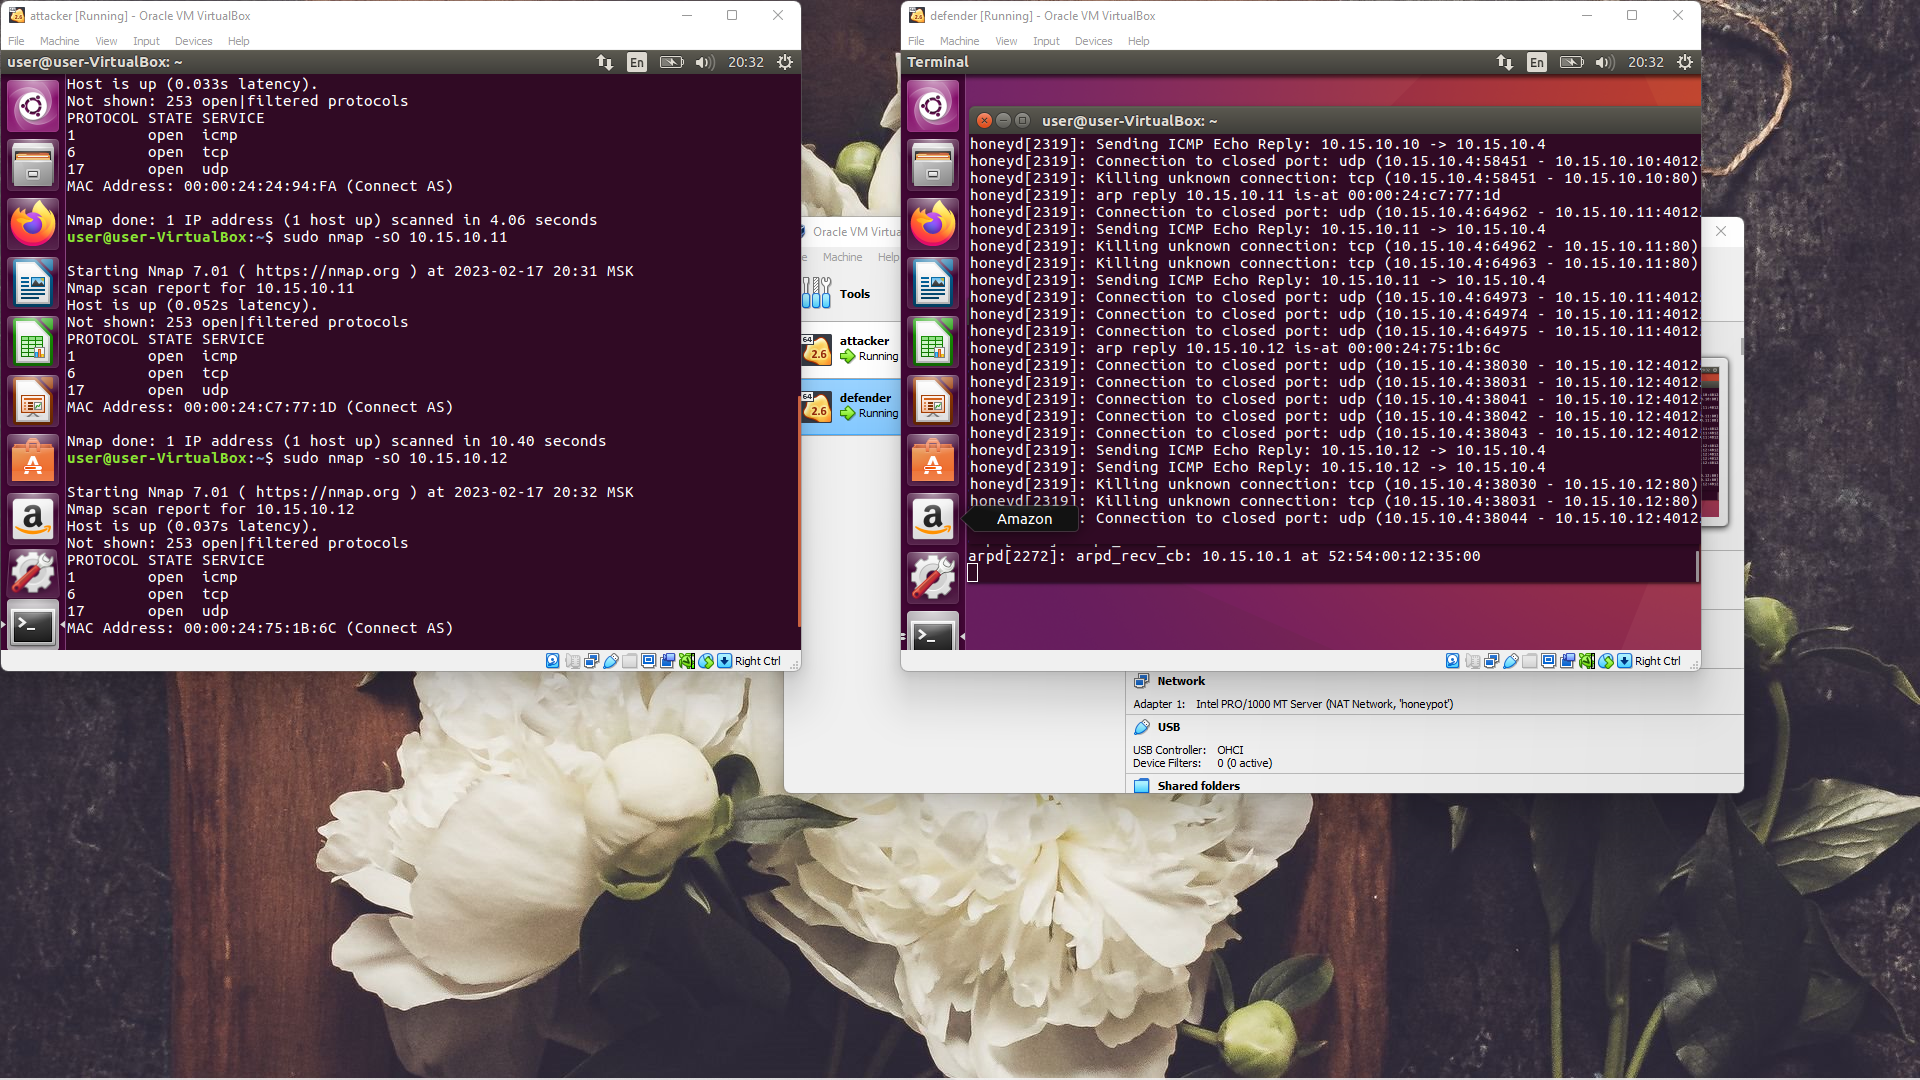
\includegraphics[width=0.85\textwidth]{01_00 (29)}
    \caption{Сканирование IP протоколов}
  \end{figure}

  Как видно из результатов данного сканирования, каждый из настроенных
  хостов принимает \textit{UPD}, \textit{TCP} и \textit{ICMP} пакеты.

  \subsubsection{ACK-сканирование}

  \begin{figure}[H]
    \centering
    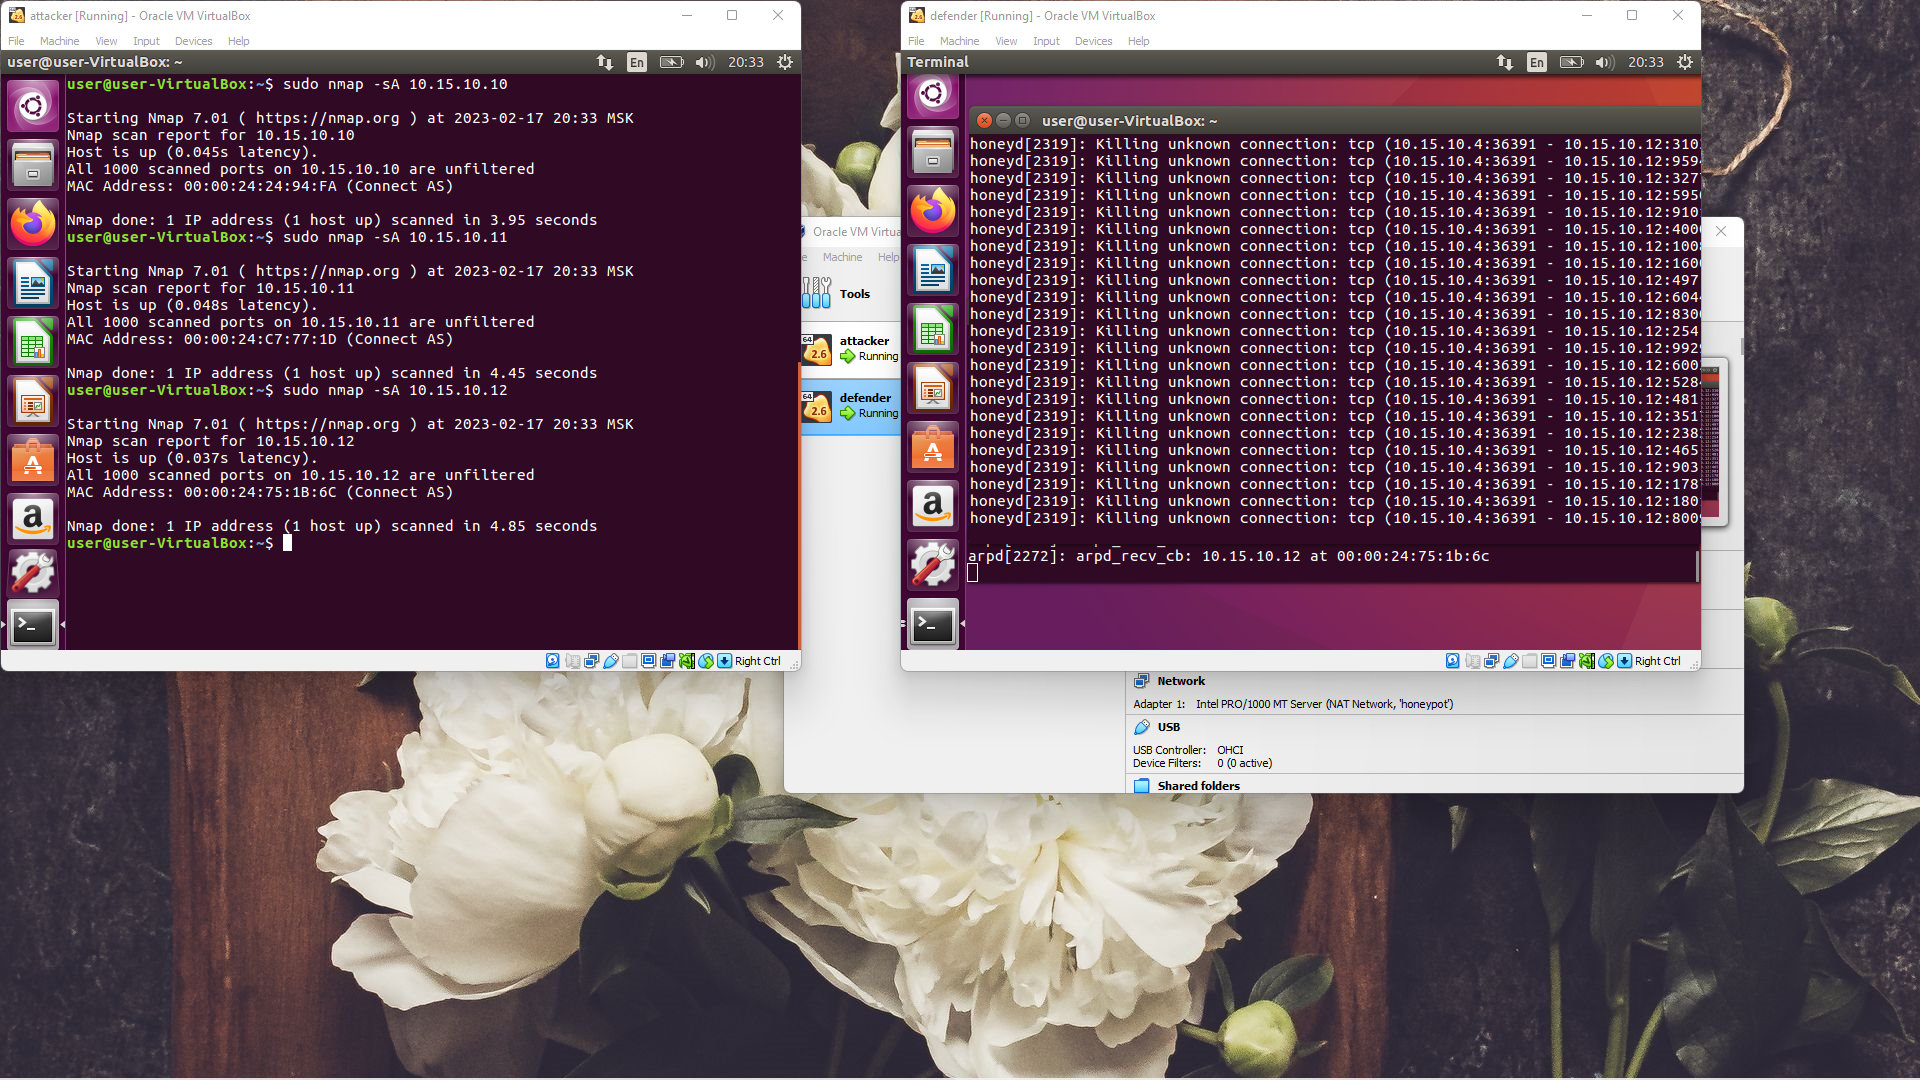
\includegraphics[width=0.85\textwidth]{01_00 (30)}
    \caption{ACK-сканирование}
  \end{figure}
  
  Из результатов данного сканирования видно, что все порты на целевых машинах
  нефильтруемый.

  \subsubsection{TCP Window сканирование}

  \begin{figure}[H]
    \centering
    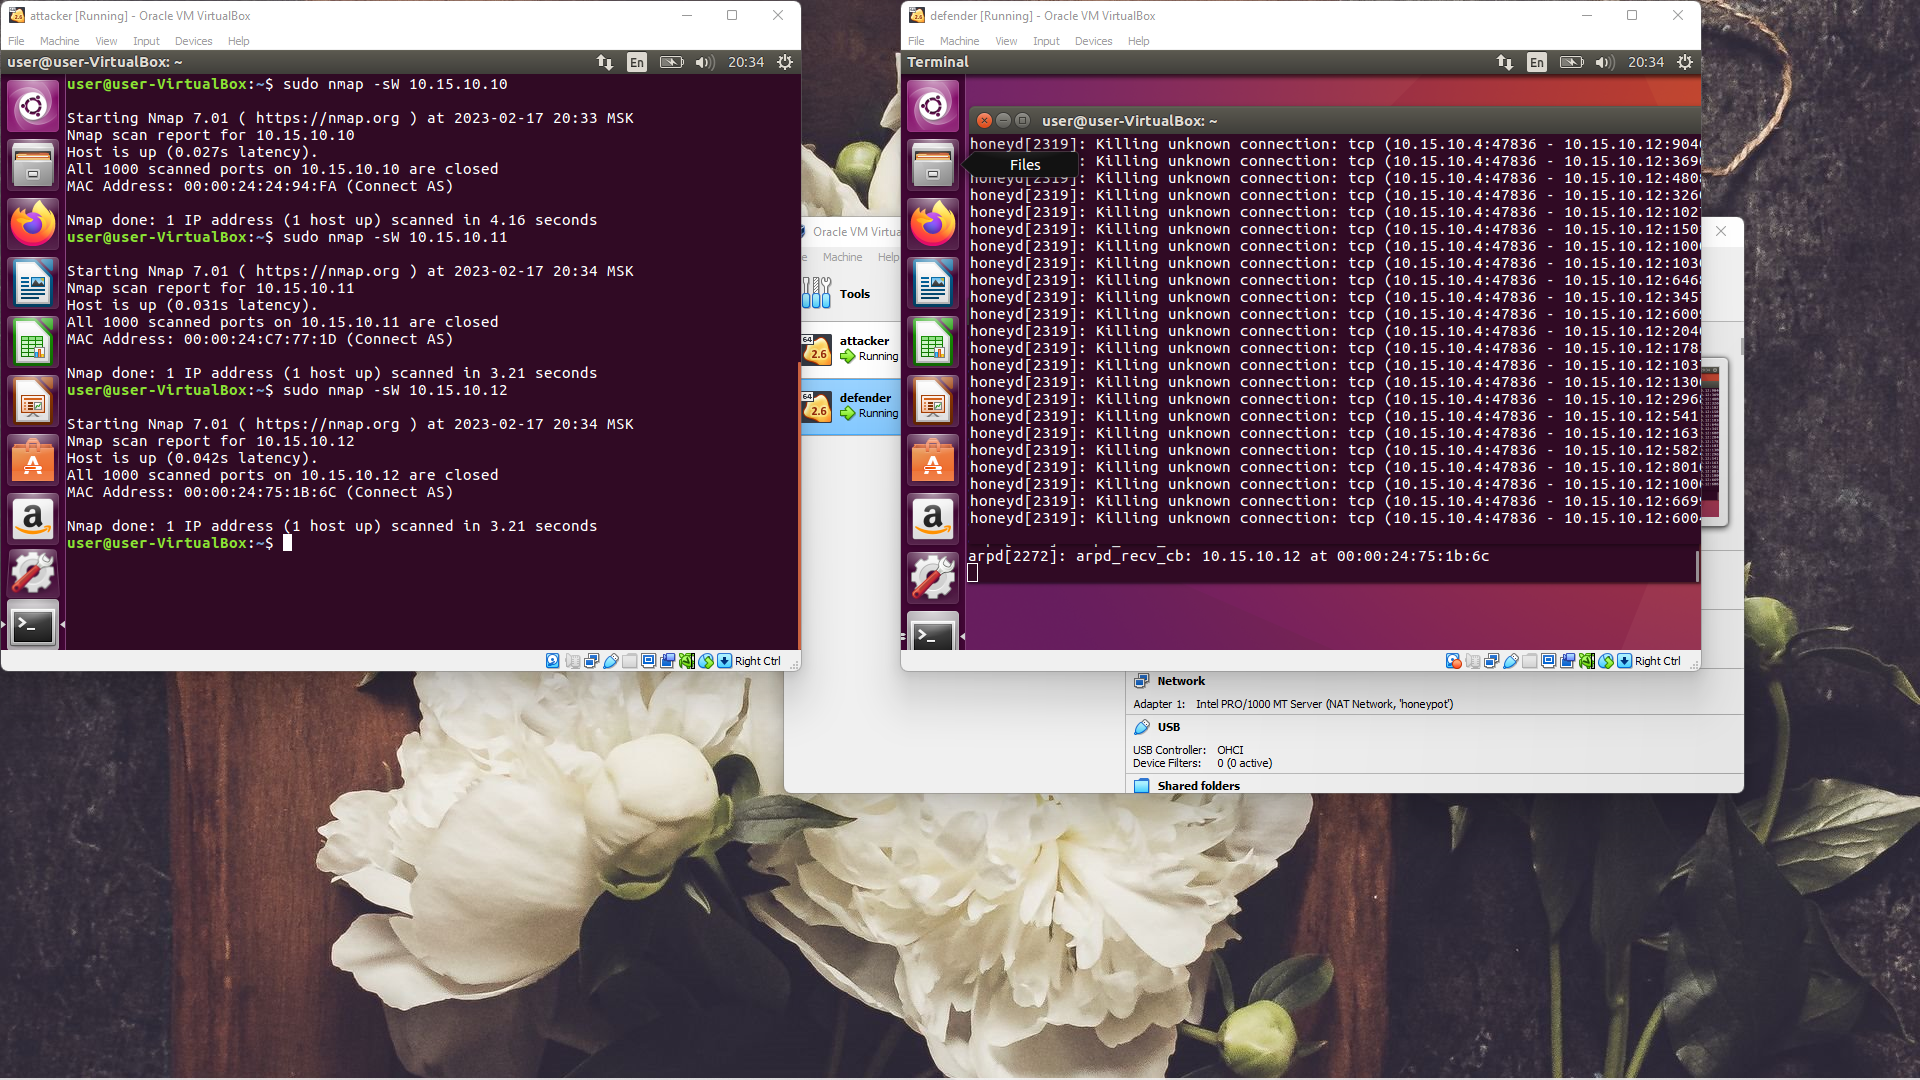
\includegraphics[width=0.85\textwidth]{01_00 (31)}
    \caption{TCP Window сканирование}
  \end{figure}

  Данный тип сканирования не увидел открытых портов.

  \subsubsection{RPC сканирование}

  \begin{figure}[H]
    \centering
    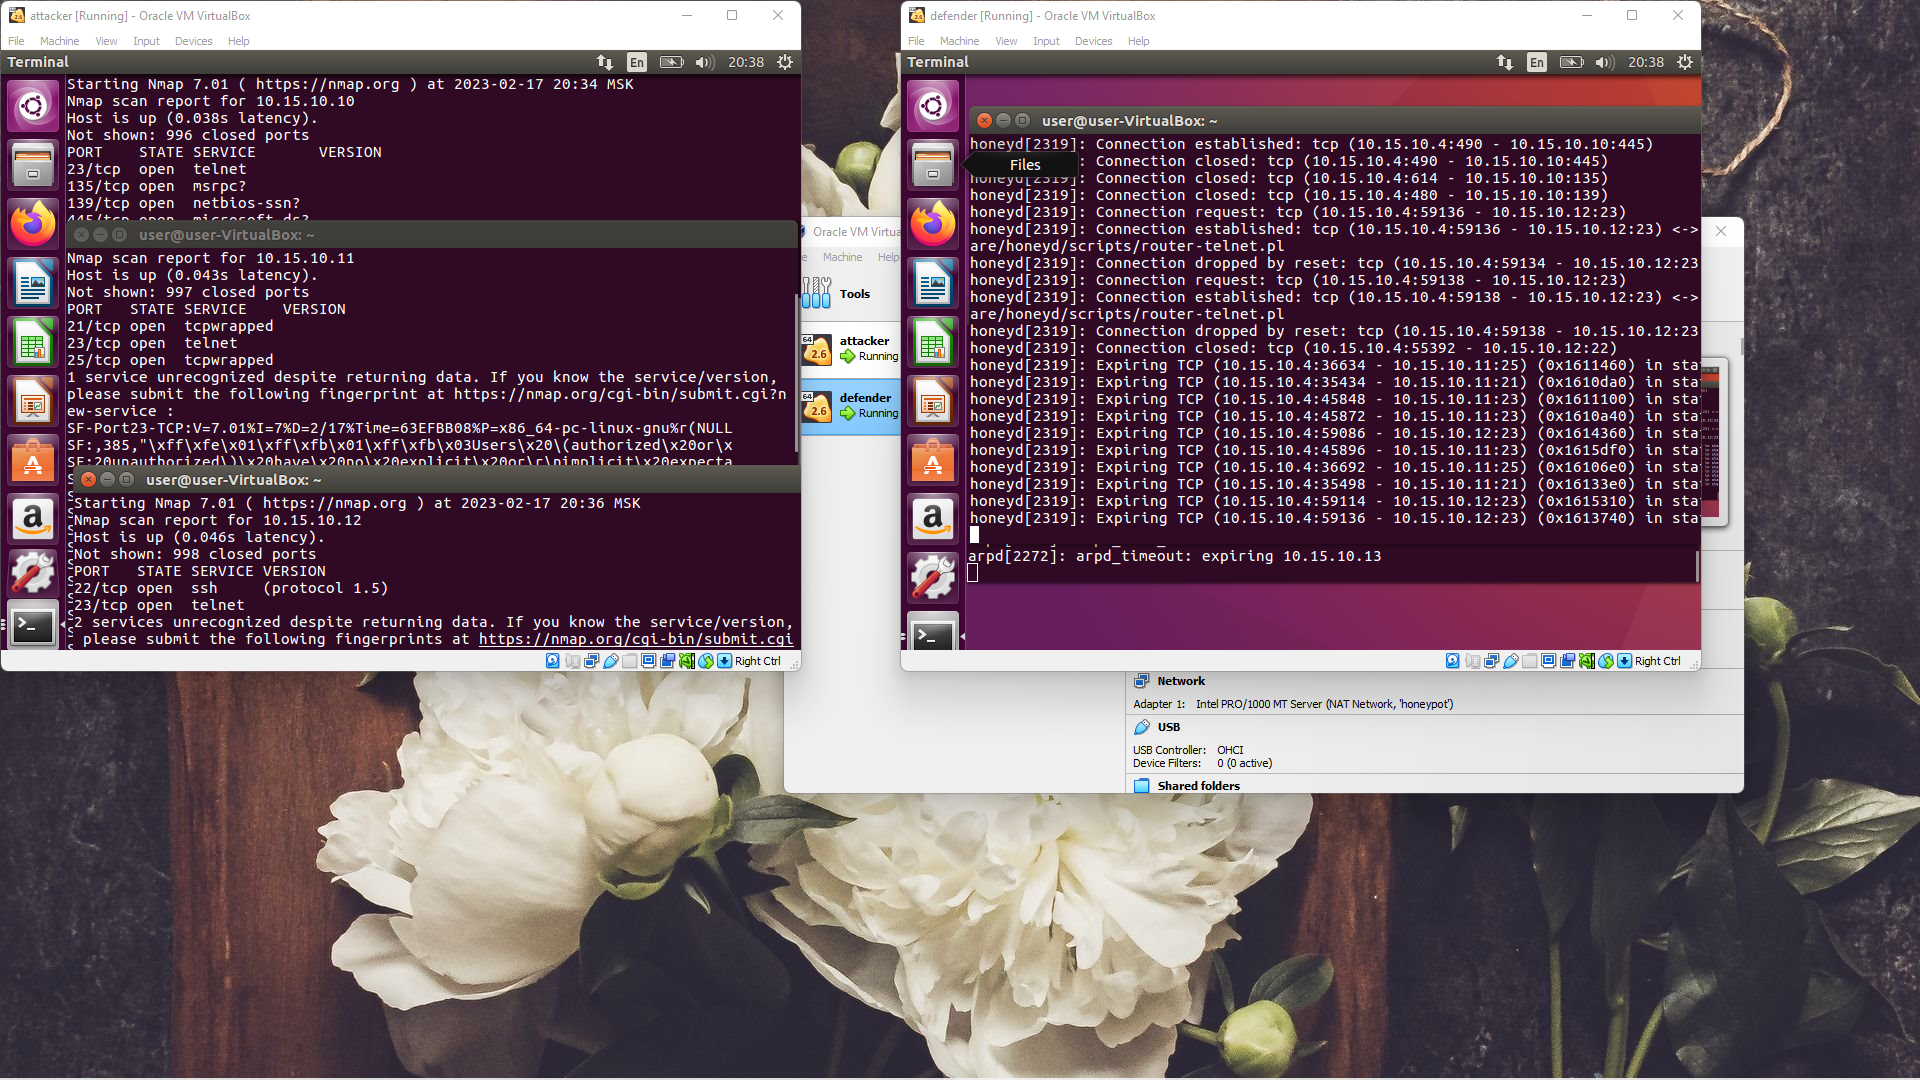
\includegraphics[width=0.85\textwidth]{01_00 (32)}
    \caption{Сканирование IP протоколов}
  \end{figure}

  Данное сканирование позволяет определить, какие программы по факту обслуживают
  те или иные порты.

  \subsubsection{Сканирование ОС}

  \begin{figure}[H]
    \centering
    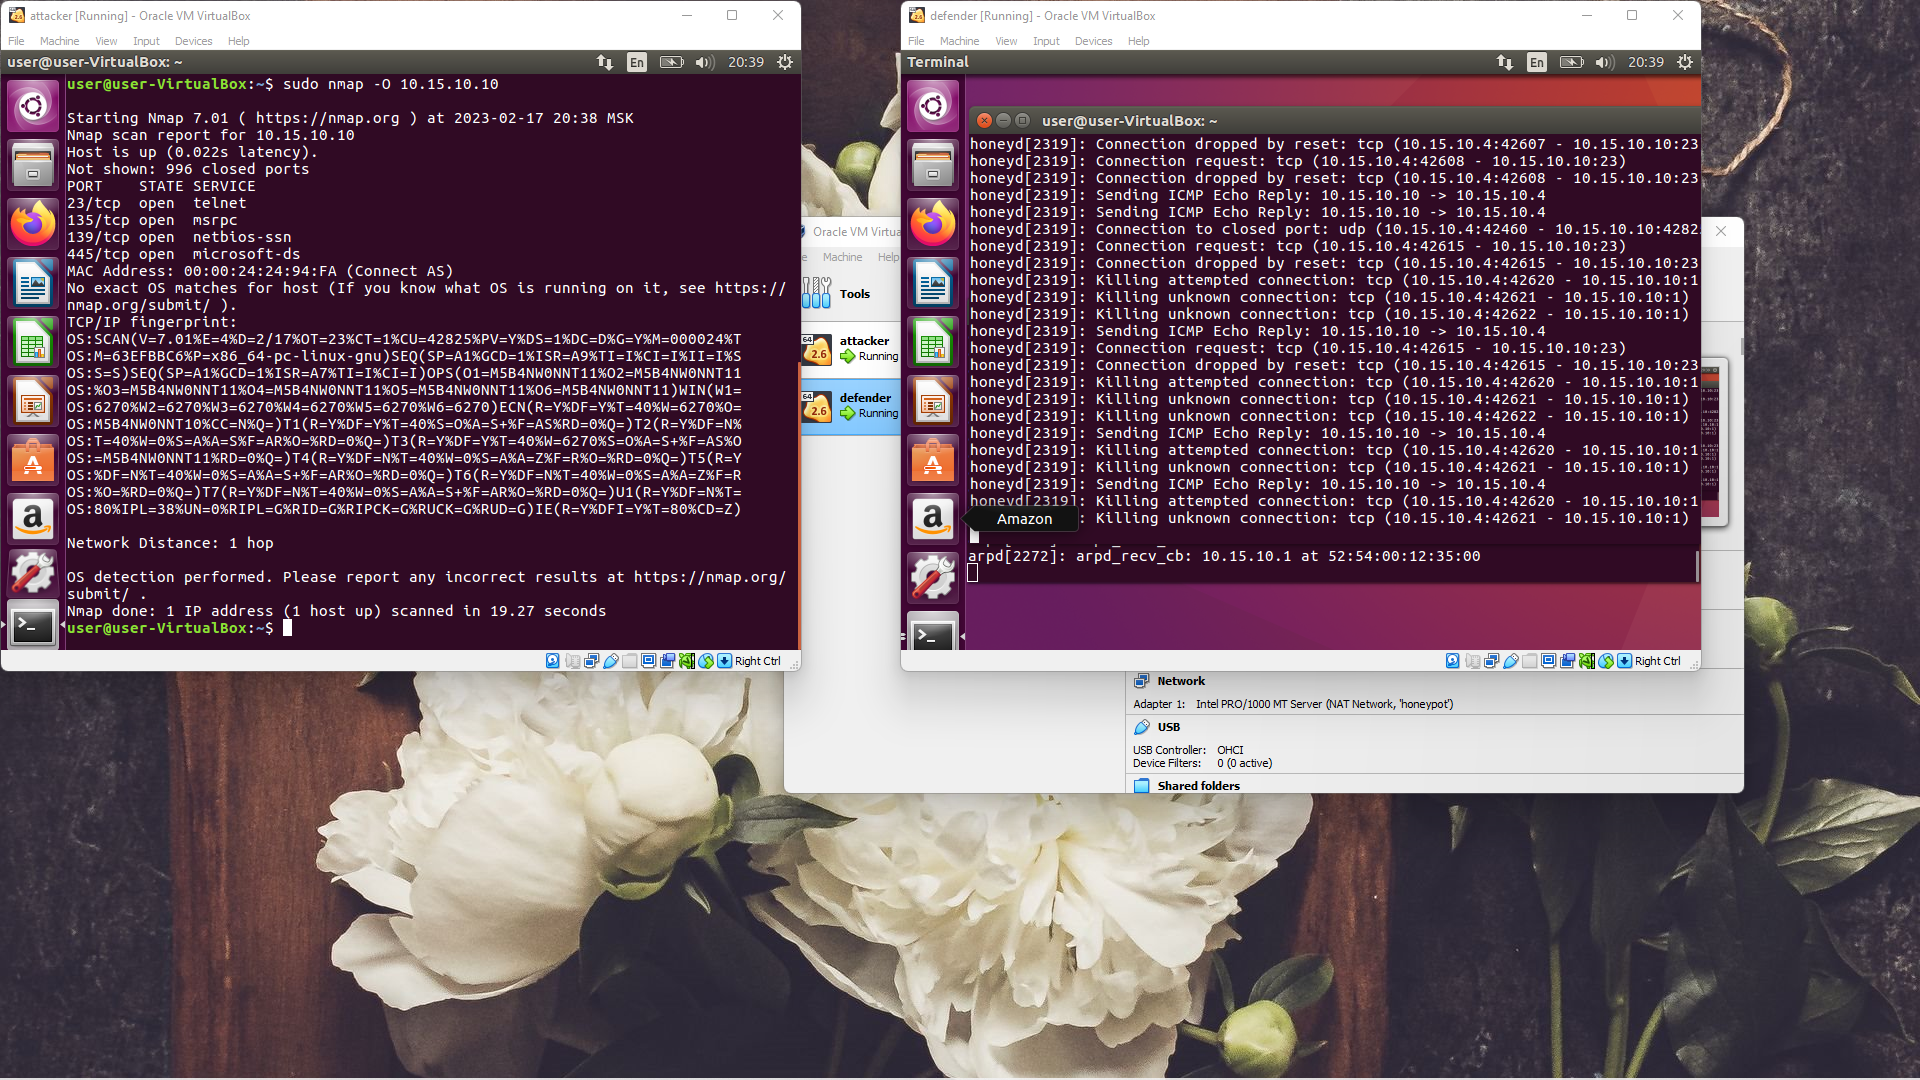
\includegraphics[width=0.85\textwidth]{01_00 (33)}
    \caption{Первая часть сканирования}
  \end{figure}

  \begin{figure}[H]
    \centering
    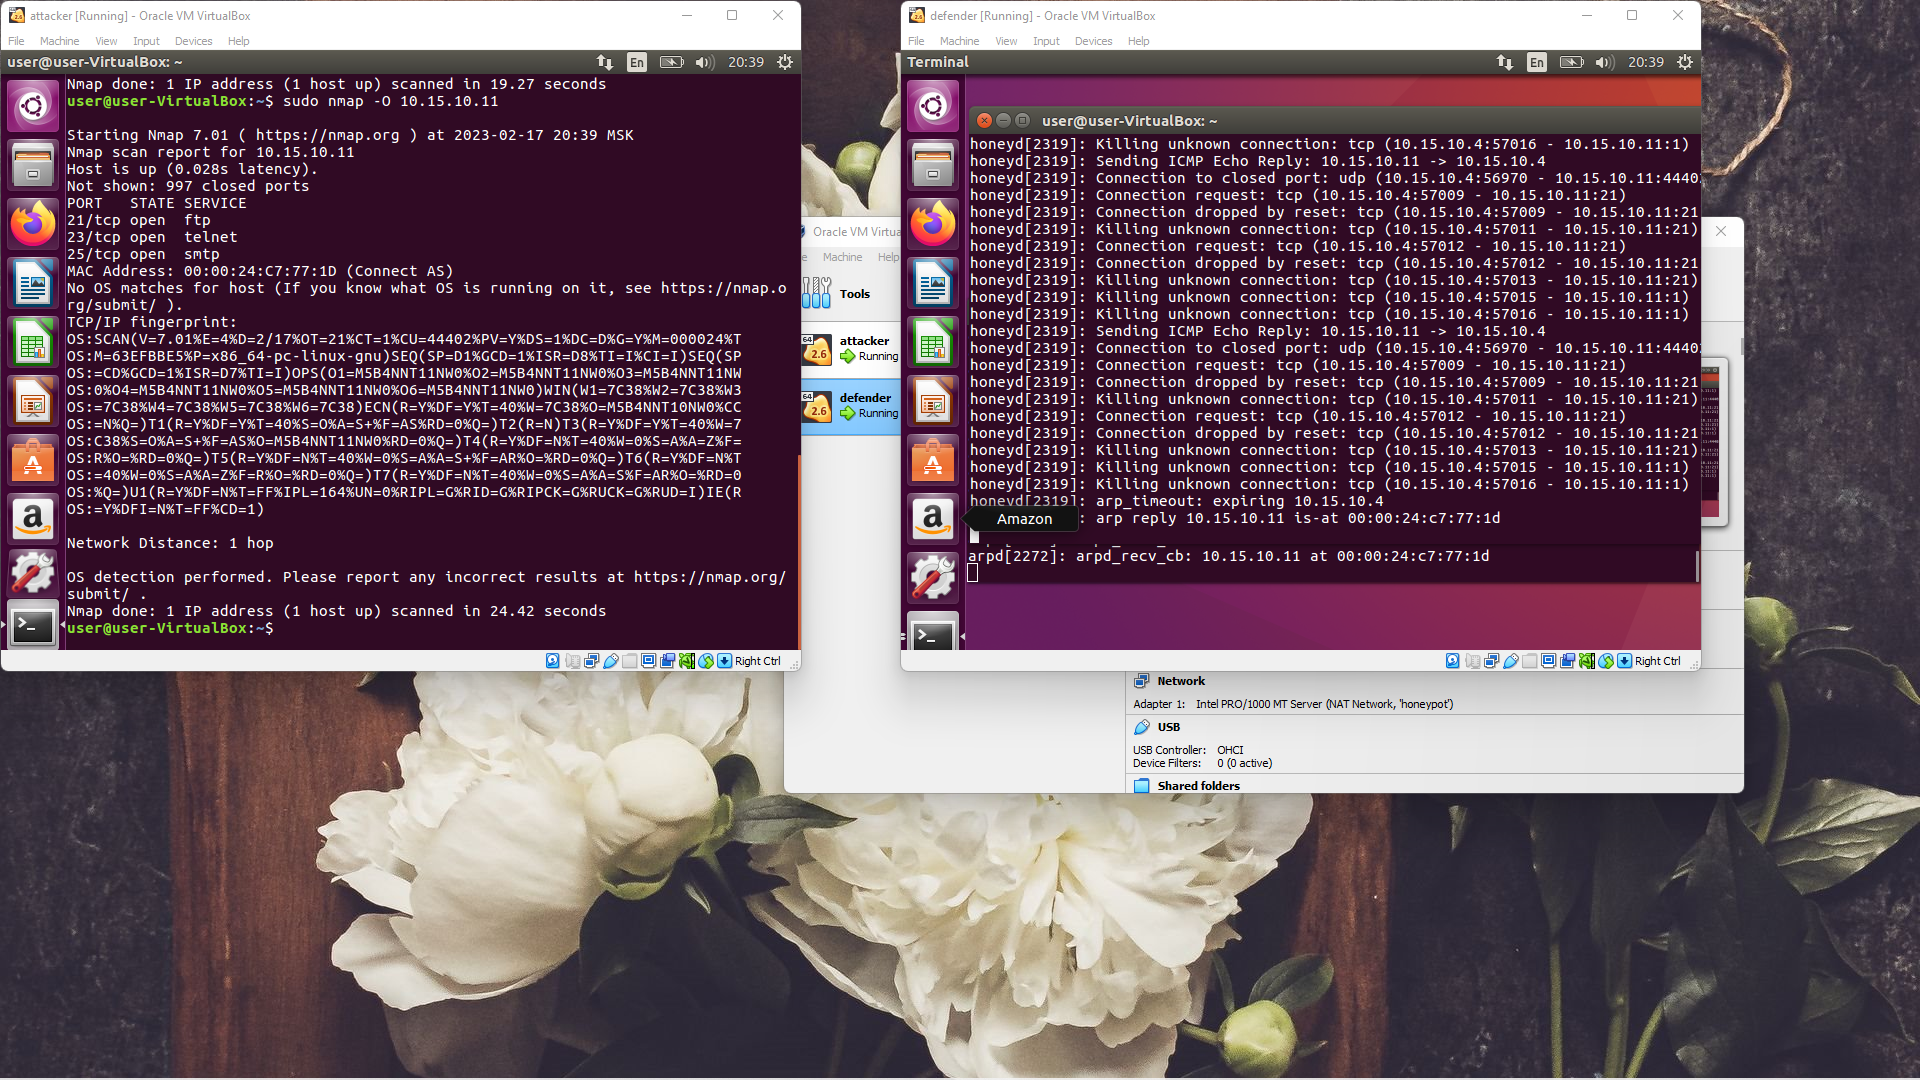
\includegraphics[width=0.85\textwidth]{01_00 (34)}
    \caption{Вторая часть сканирования}
  \end{figure}

  \begin{figure}[H]
    \centering
    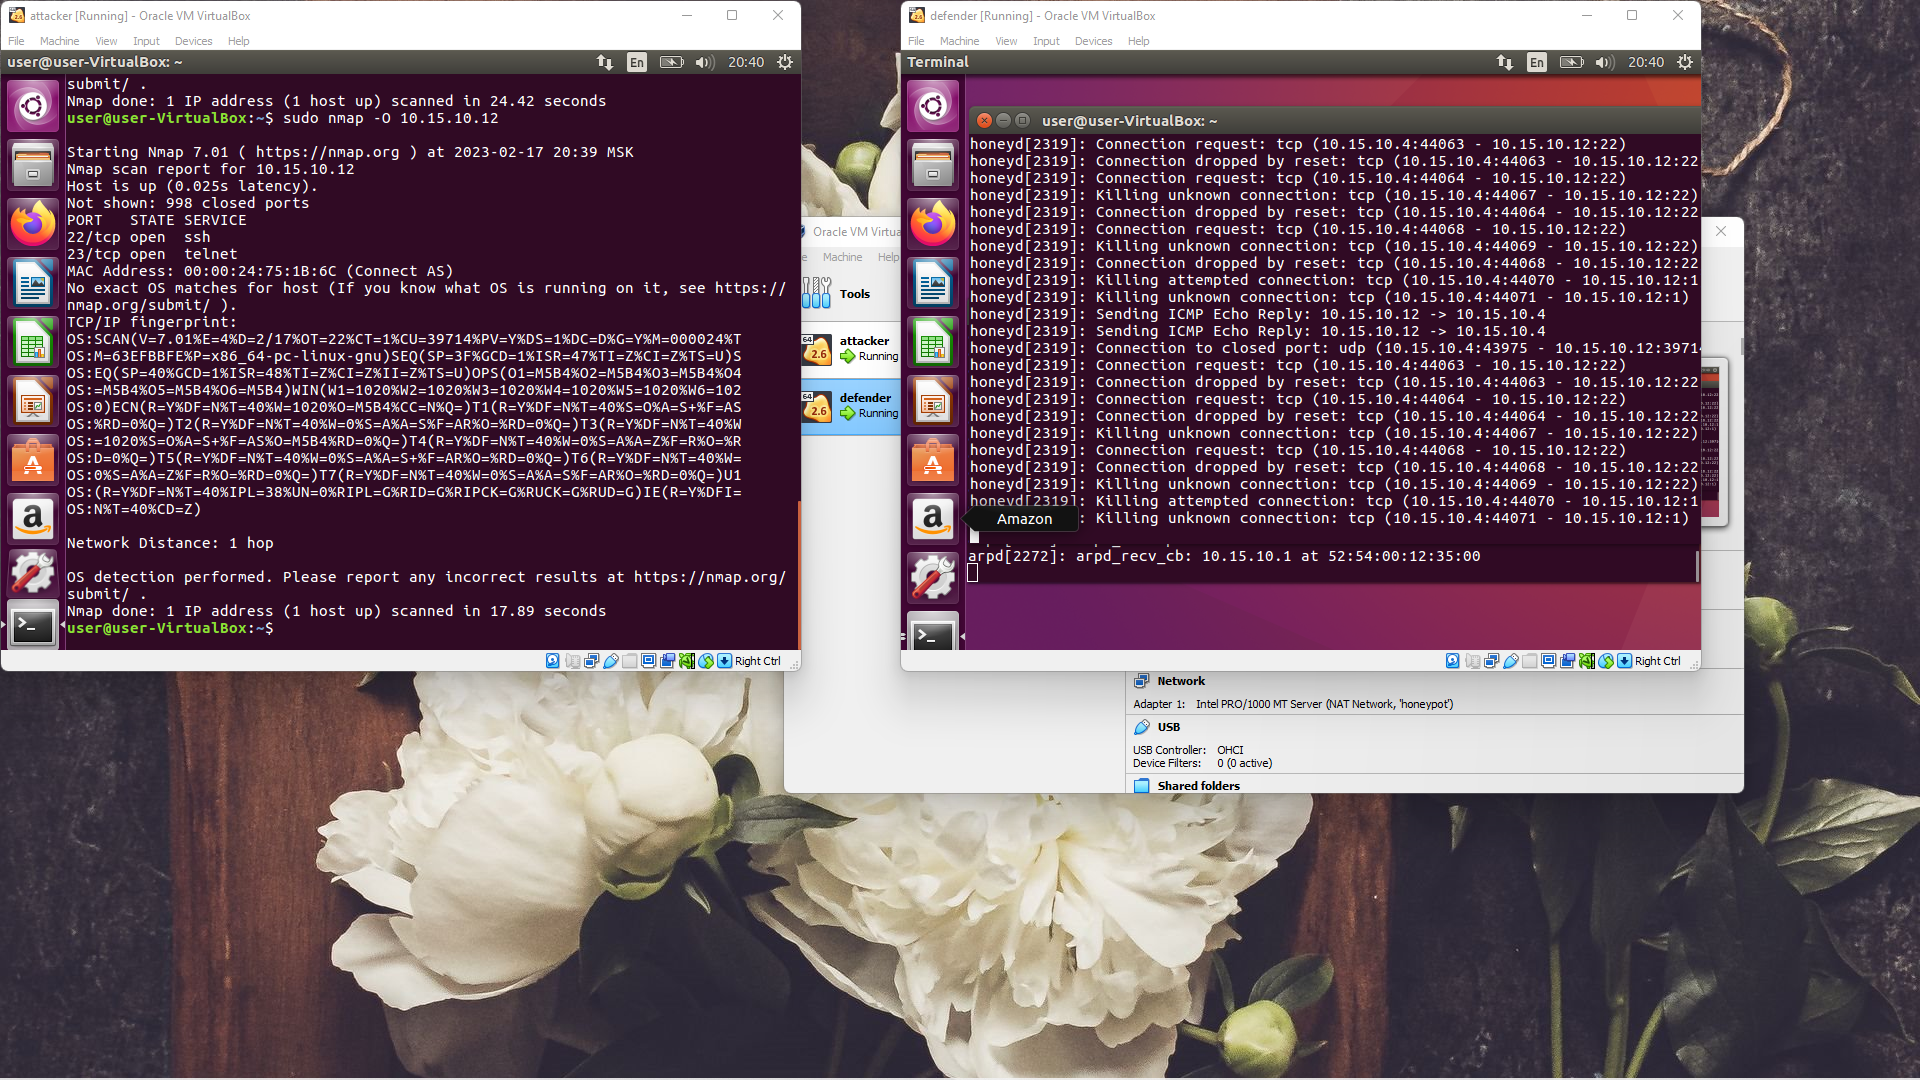
\includegraphics[width=0.85\textwidth]{01_00 (35)}
    \caption{Третья часть сканирования}
  \end{figure}

  К сожалению, \textit{nmap} не удалось определить, какие ОС эмулирует \textit{honeypot}.

  \subsubsection{NULL сканирование}

  \begin{figure}[H]
    \centering
    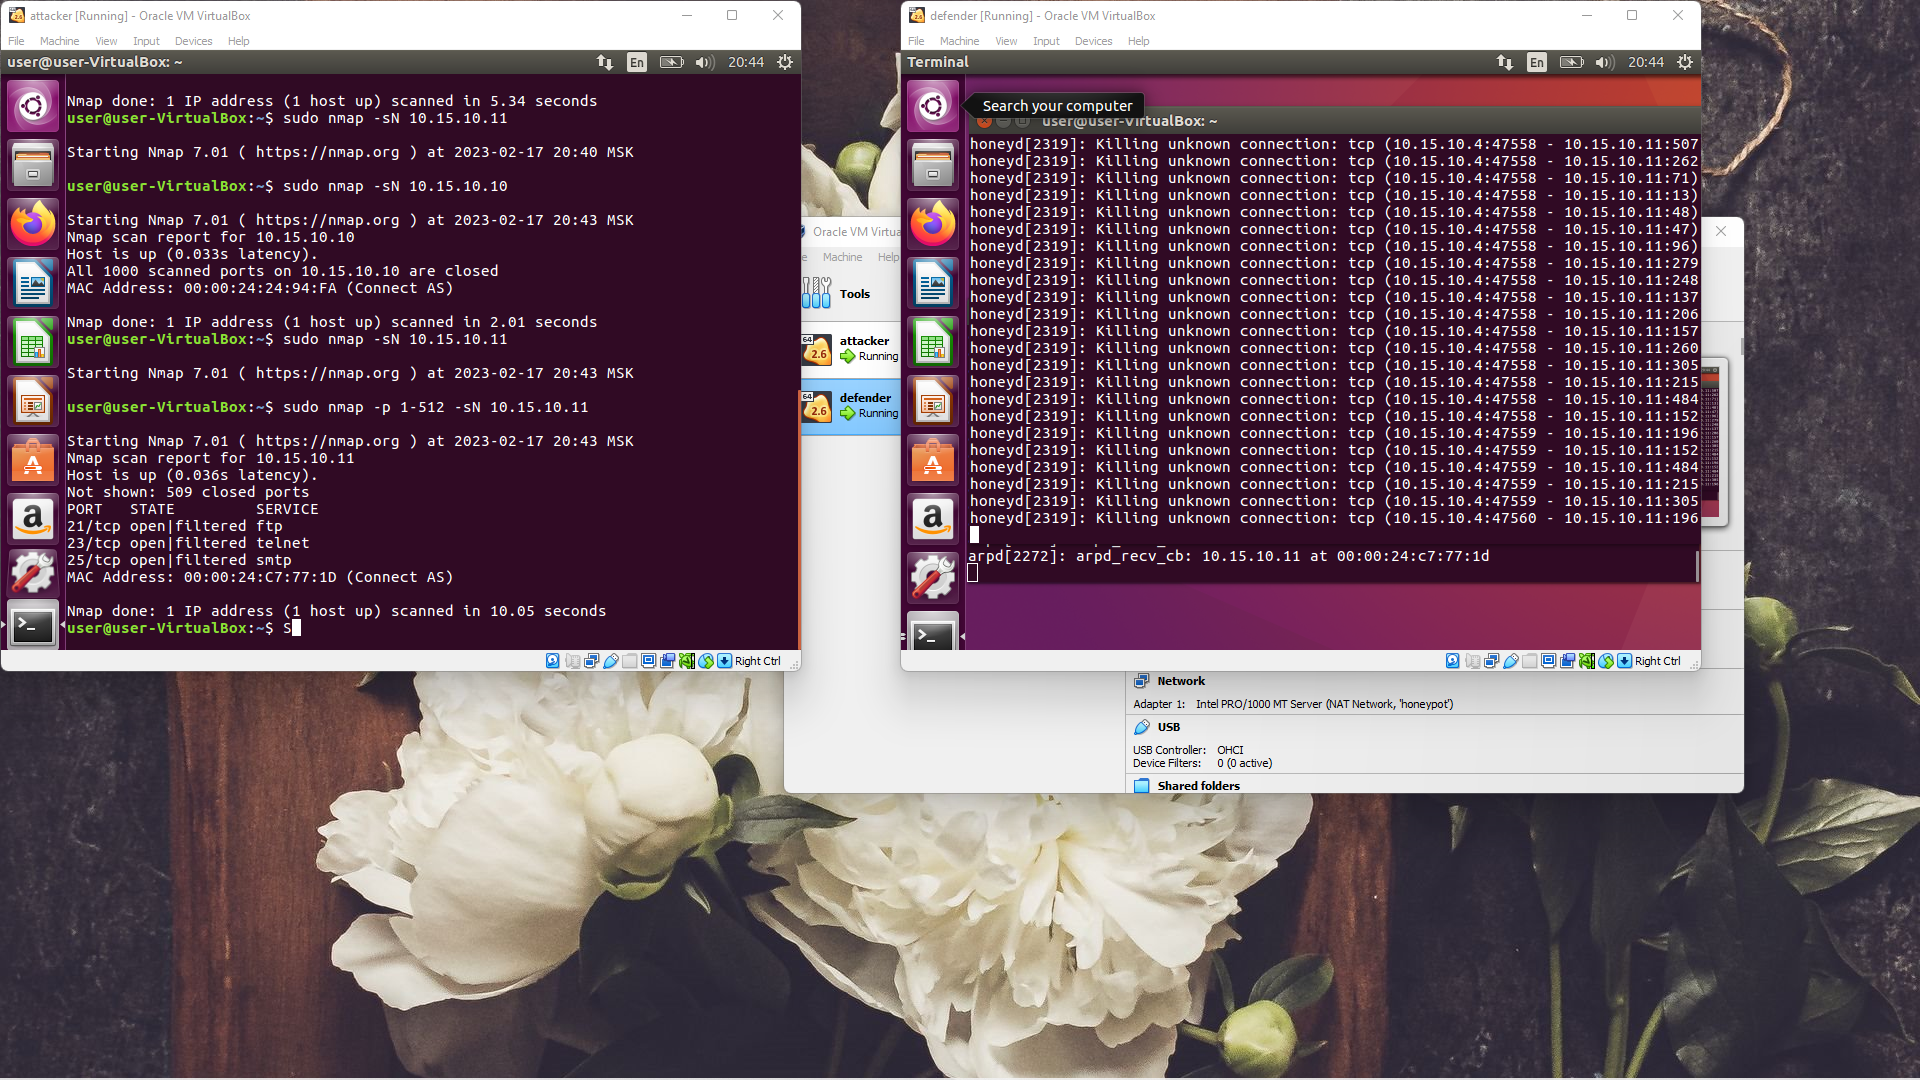
\includegraphics[width=0.85\textwidth]{01_00 (37)}
    \caption{Сканирование NULL}
  \end{figure}

  Для некоторых \textit{IP} адресов \textit{nmap} определил \textit{MAC} адреса.
  А где-то еще и фильтруемость портов.

  \subsubsection{FIN сканирование}

  \begin{figure}[H]
    \centering
    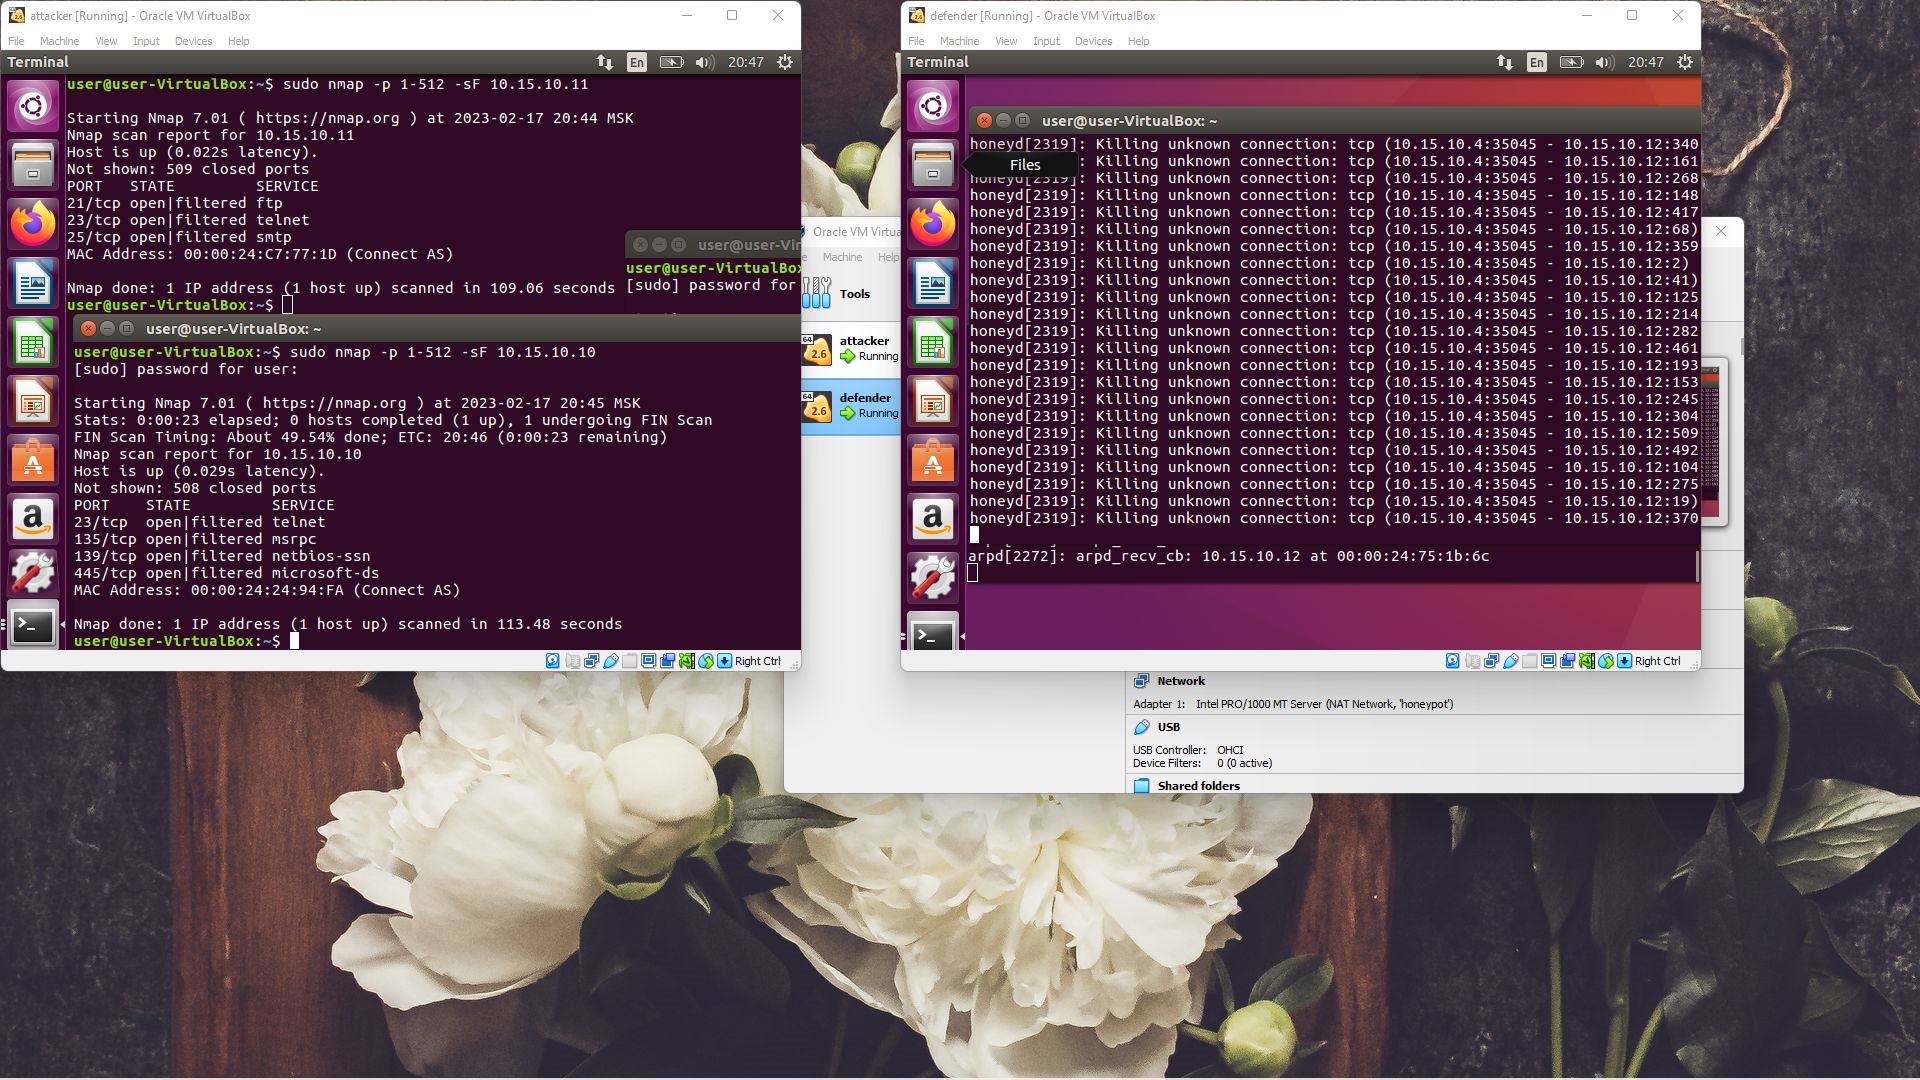
\includegraphics[width=0.85\textwidth]{01_00 (38)}
    \caption{Первая часть сканирования}
  \end{figure}

  \begin{figure}[H]
    \centering
    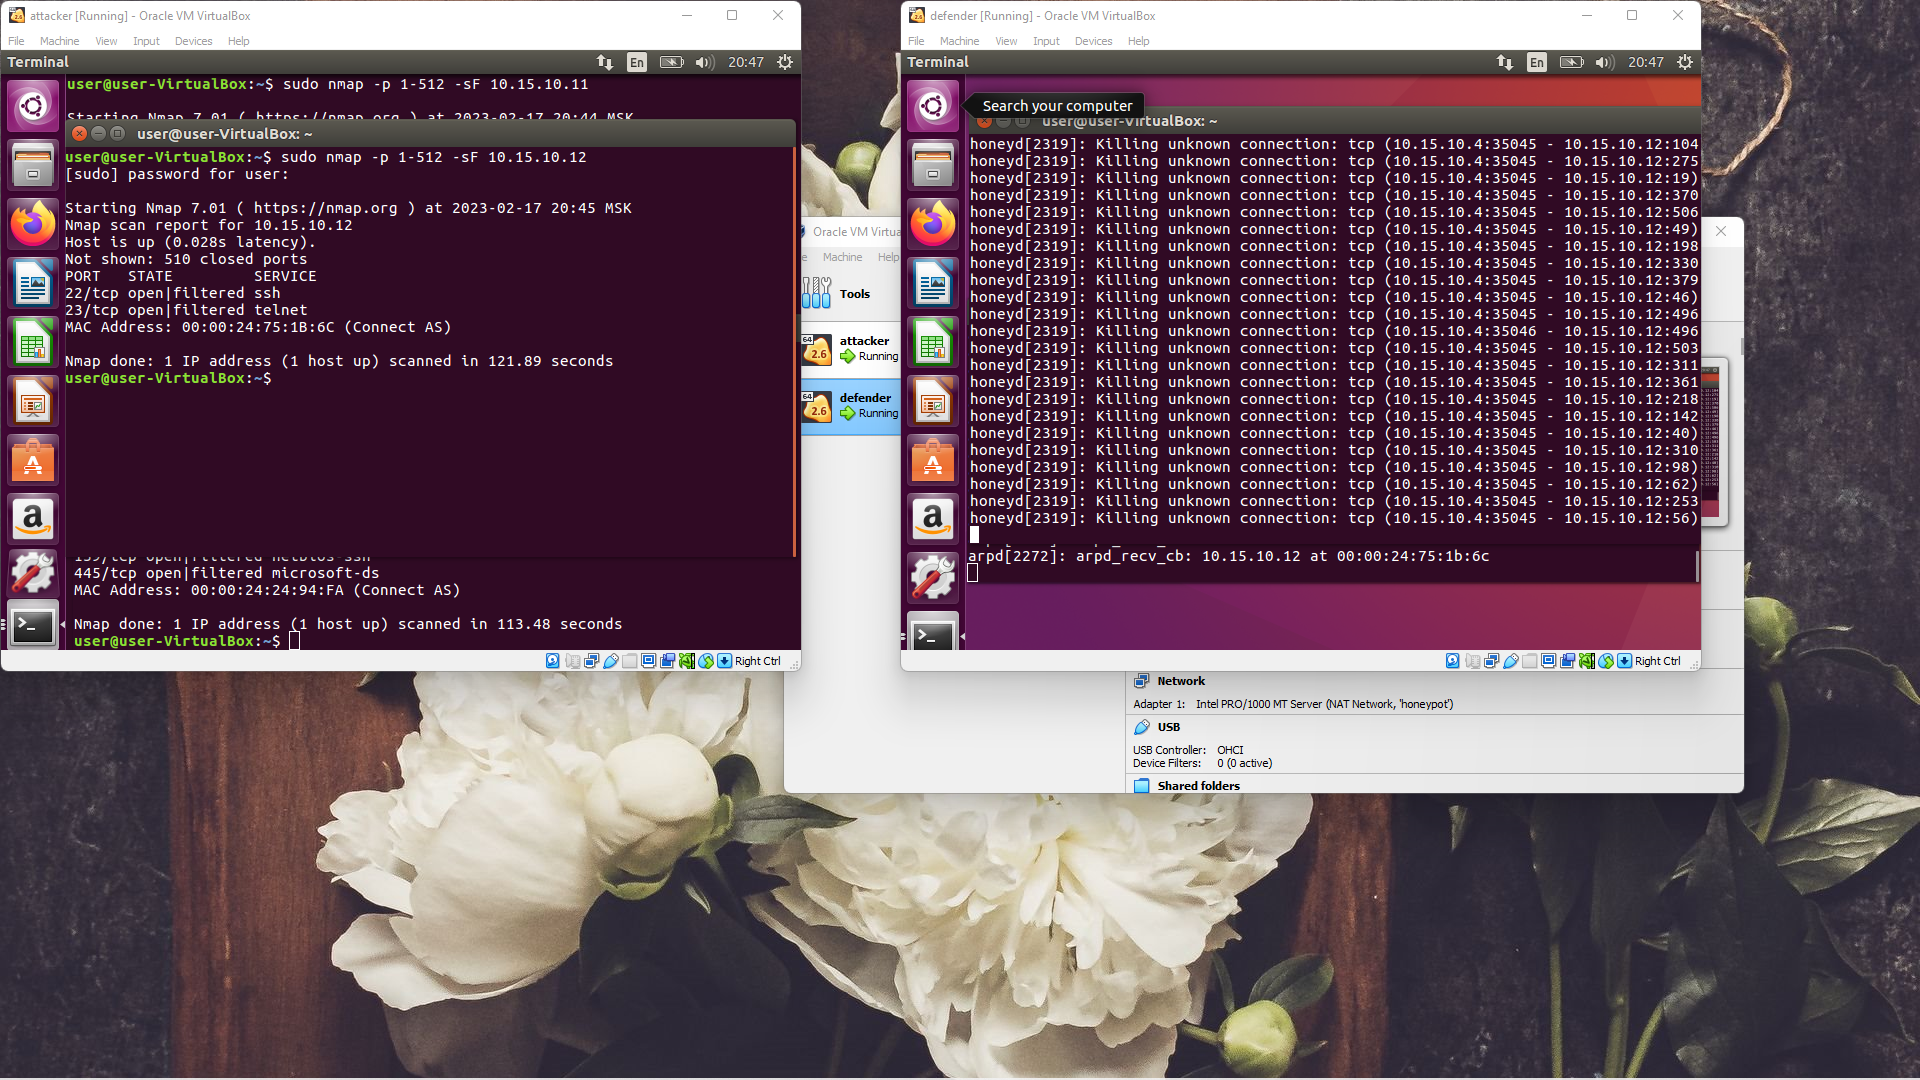
\includegraphics[width=0.85\textwidth]{01_00 (39)}
    \caption{Вторая часть сканирования}
  \end{figure}

  \subsubsection{XMas сканирование}
  \begin{figure}[H]
    \centering
    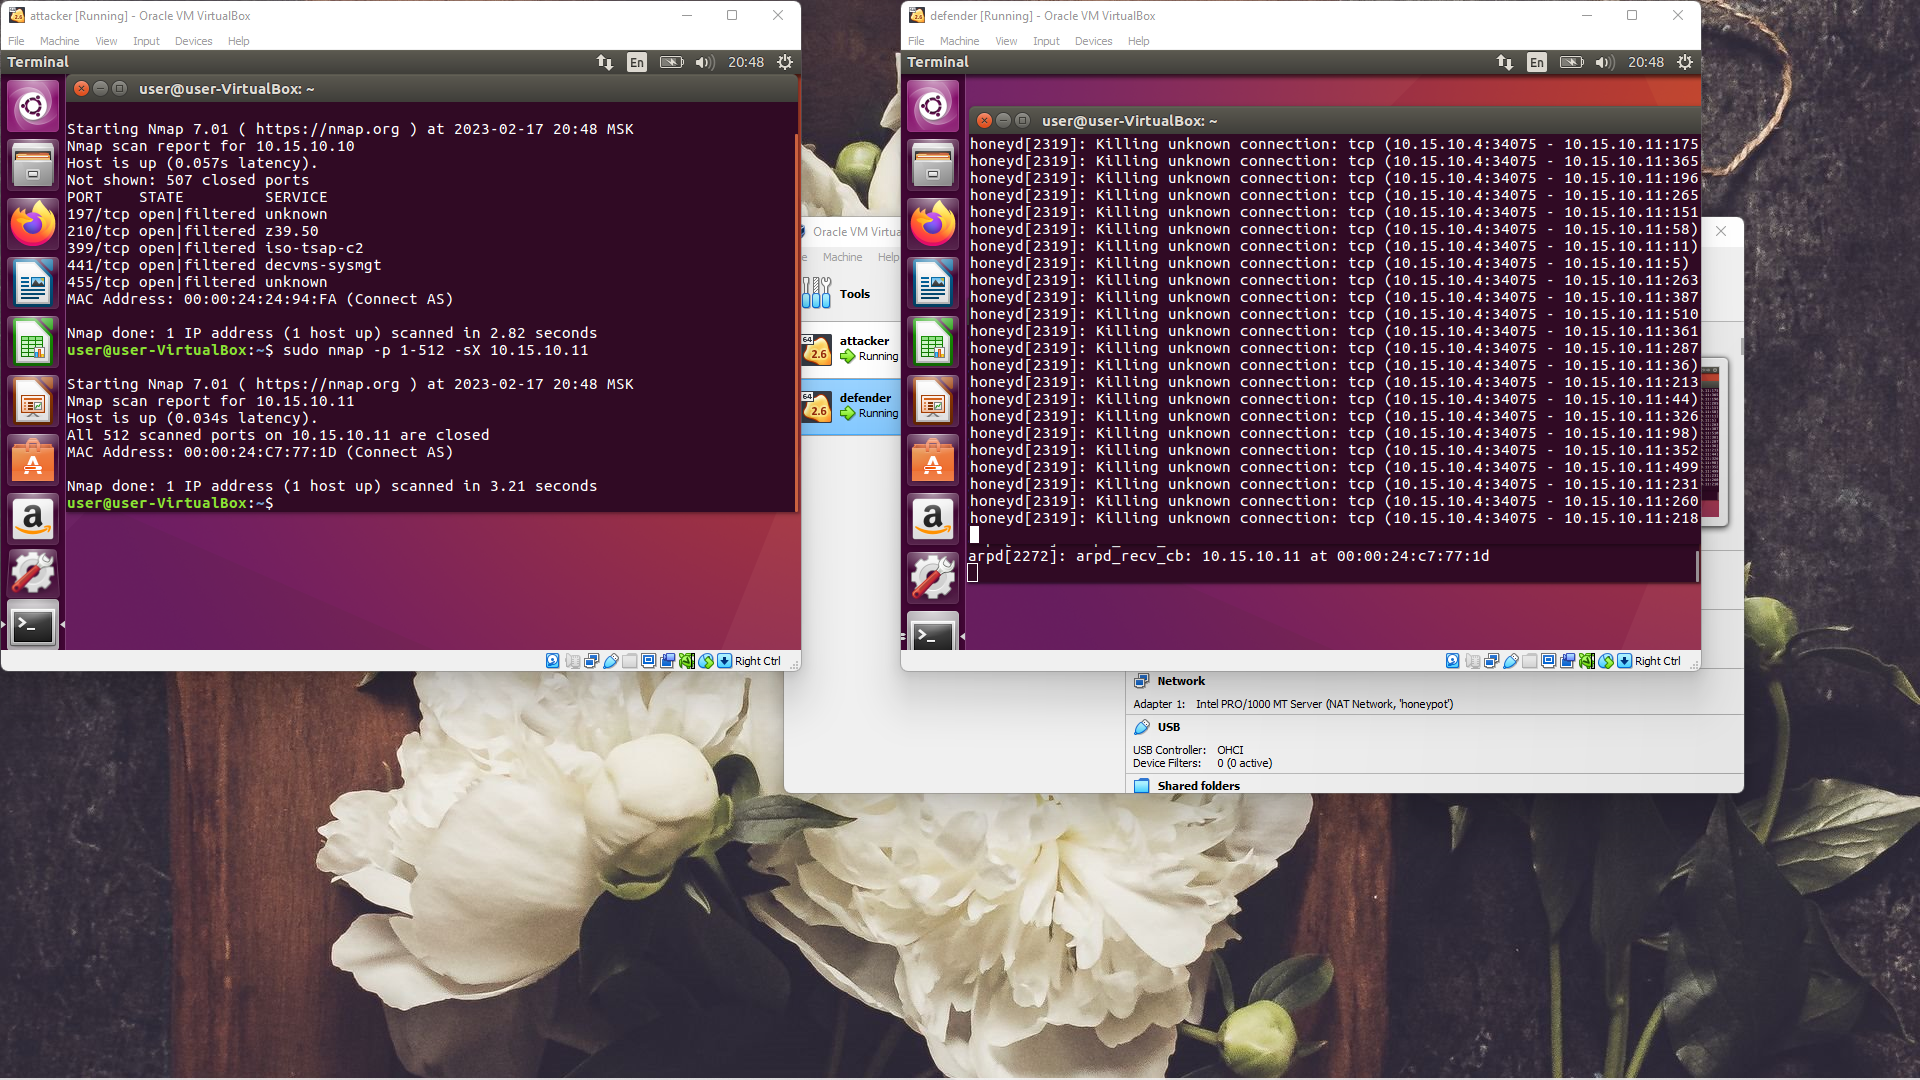
\includegraphics[width=0.85\textwidth]{01_00 (41)}
    \caption{Первая часть сканирования}
  \end{figure}

  \begin{figure}[H]
    \centering
    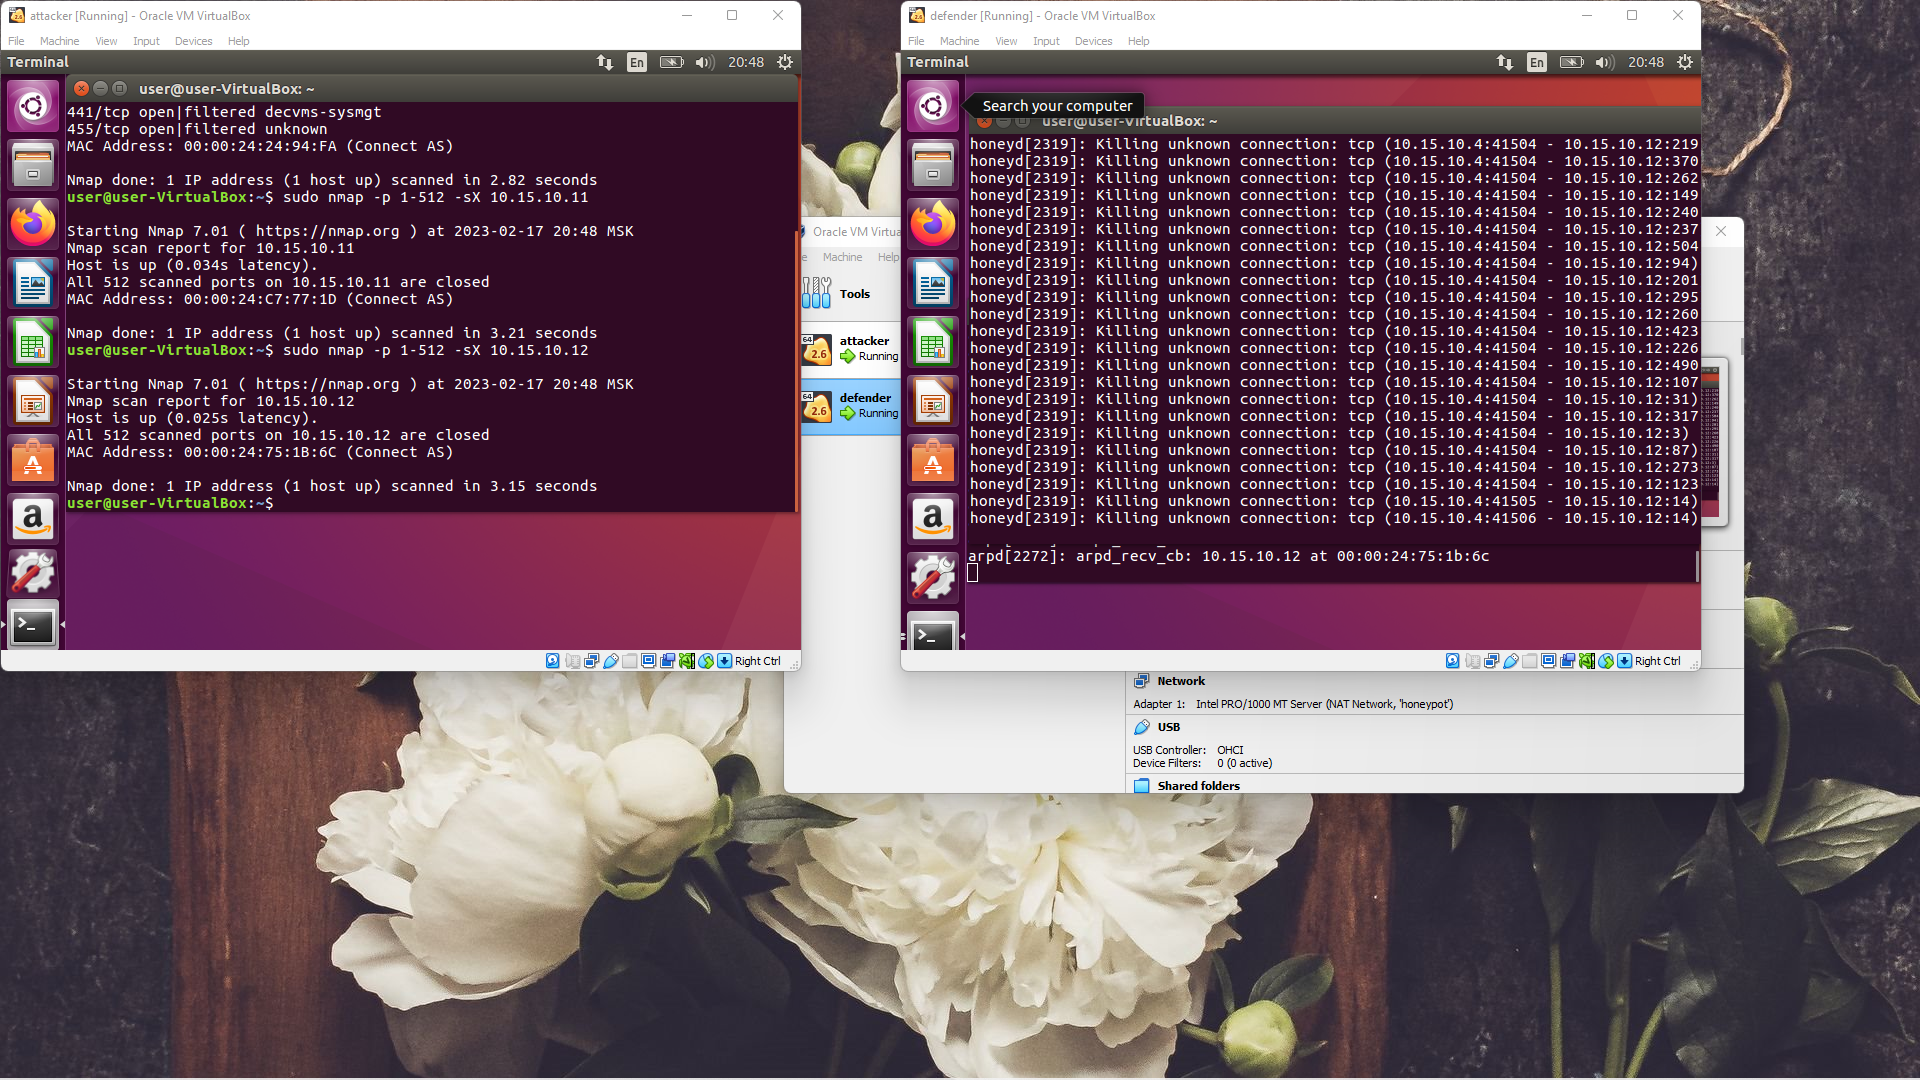
\includegraphics[width=0.85\textwidth]{01_00 (42)}
    \caption{Вторая часть сканирования}
  \end{figure}

  \subsubsection{Добавление новых ловушек}

  \begin{figure}[H]
    \centering
    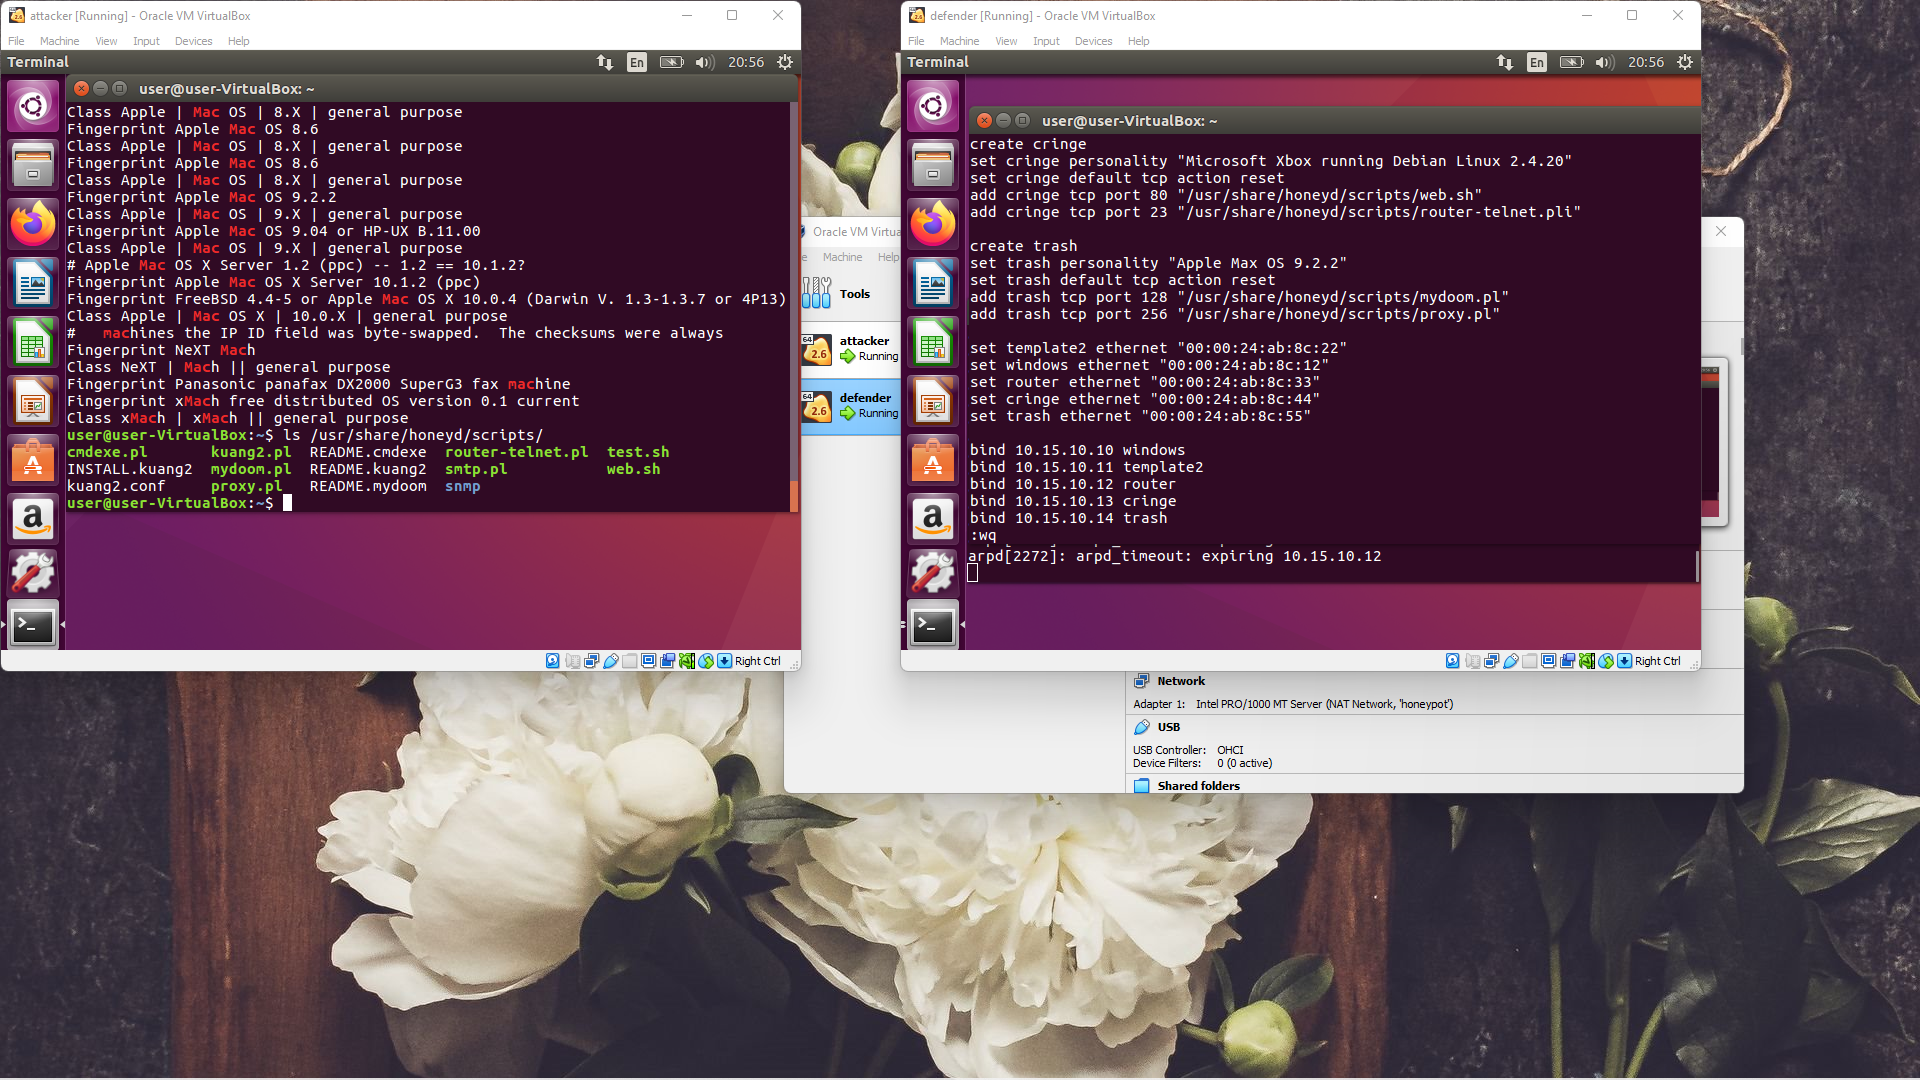
\includegraphics[width=0.85\textwidth]{01_00 (43)}
    \caption{Конфигурационный файл}
  \end{figure}

  Созданы две новые конфигруации, одна с открытыми 80 и 23 портами,
  а другая - с 128 и 256.

  \begin{figure}[H]
    \centering
    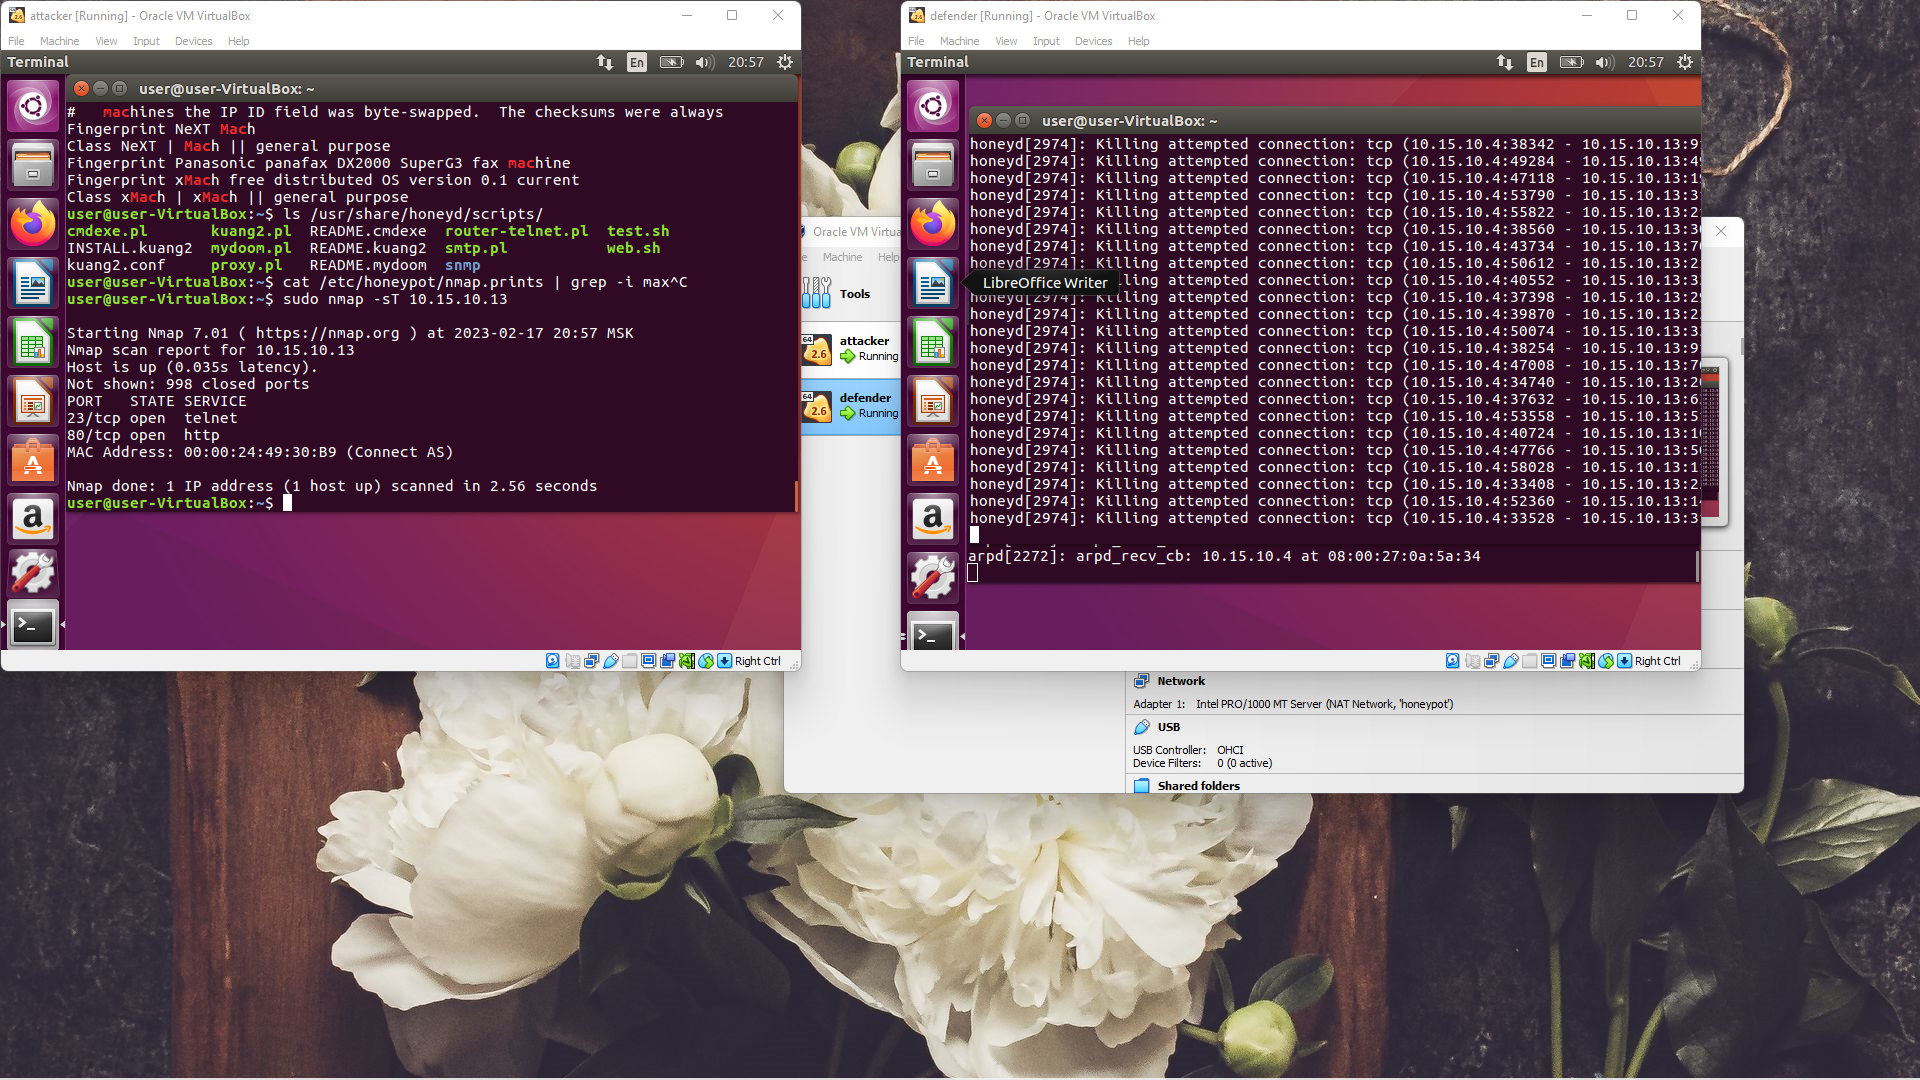
\includegraphics[width=0.85\textwidth]{01_00 (44)}
    \caption{Проверка первой ловушки}
  \end{figure}
  
  \begin{figure}[H]
    \centering
    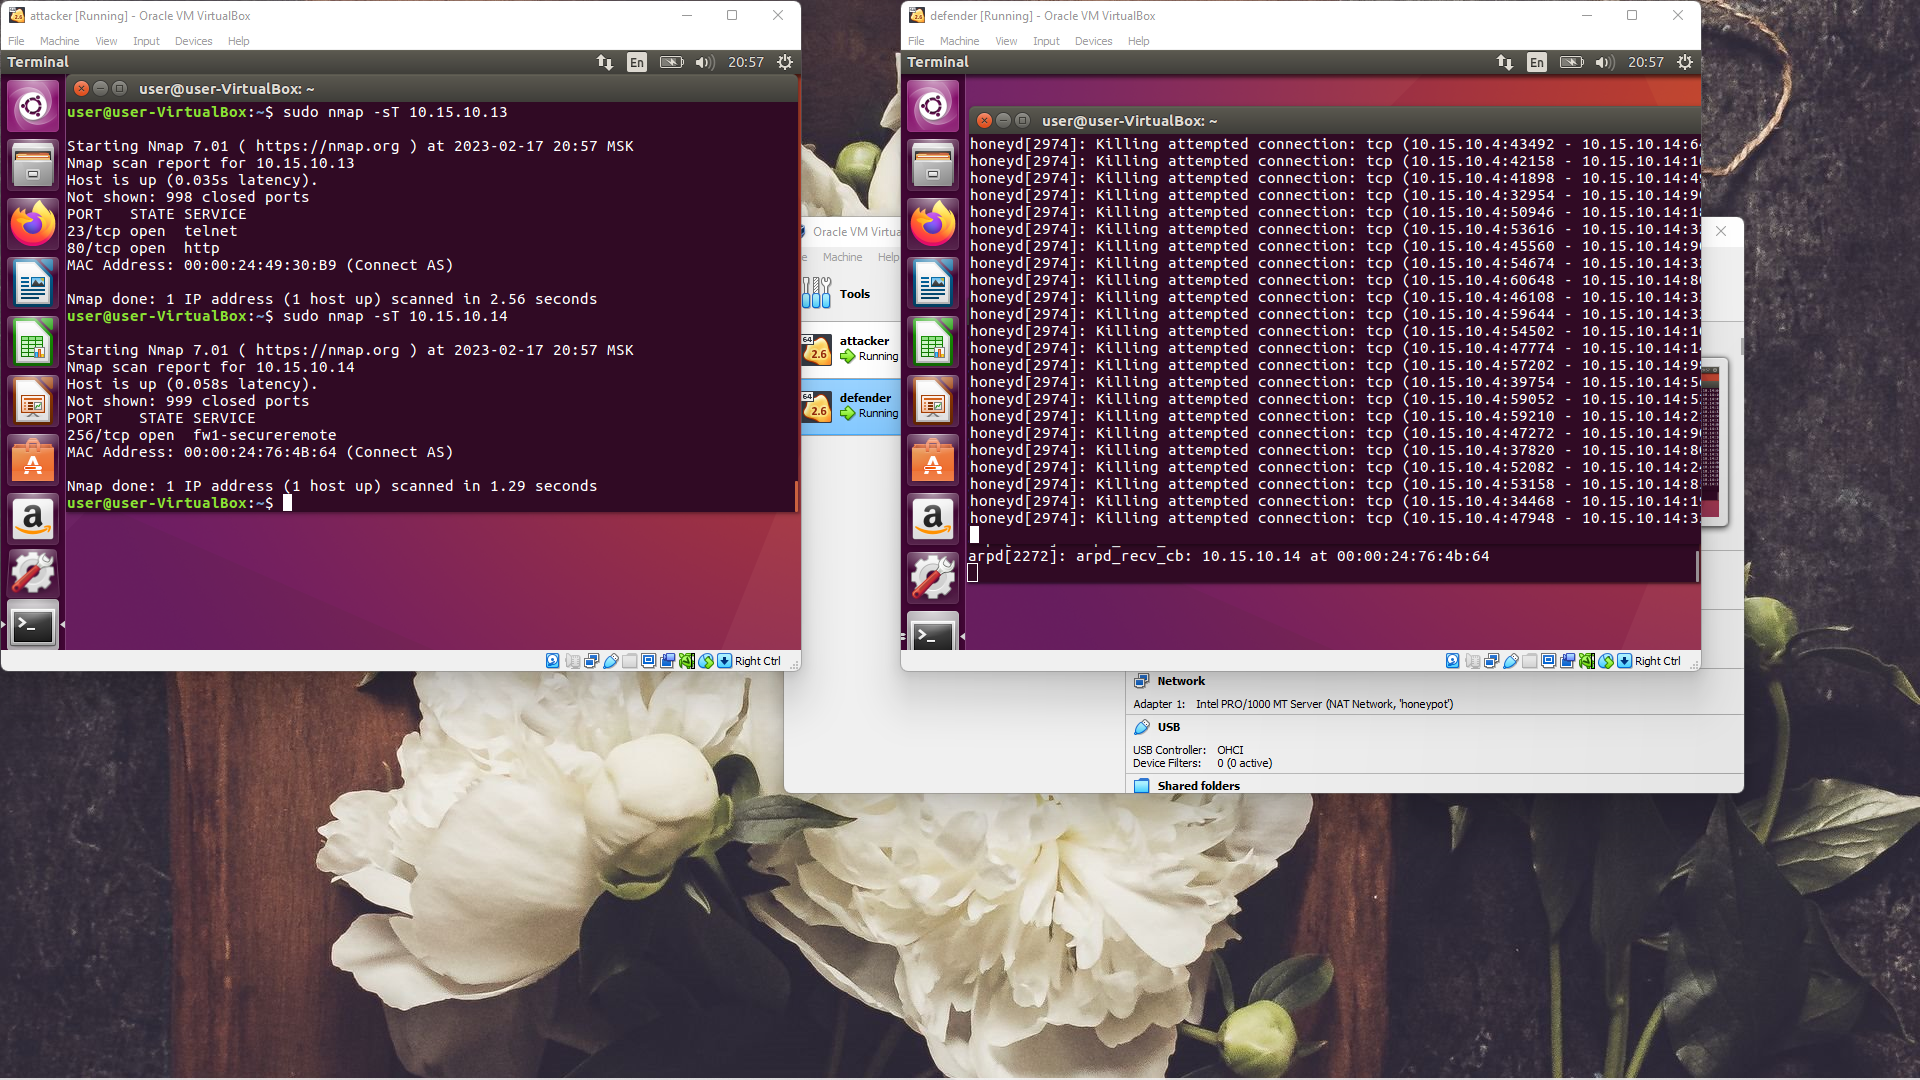
\includegraphics[width=0.85\textwidth]{01_00 (45)}
    \caption{Проверка второй ловушки}
  \end{figure}

  Созданные ловушки можно проверить через \textit{nmap} - прописанные порты будут обнаружены
  и помеченны как открытые, что и произошло на скриншотах.

  \subsection{Часть 2}

  Для начала необходимо запустить \textit{Wireshark} и начать захват пакетов:
  \begin{figure}[H]
    \centering
    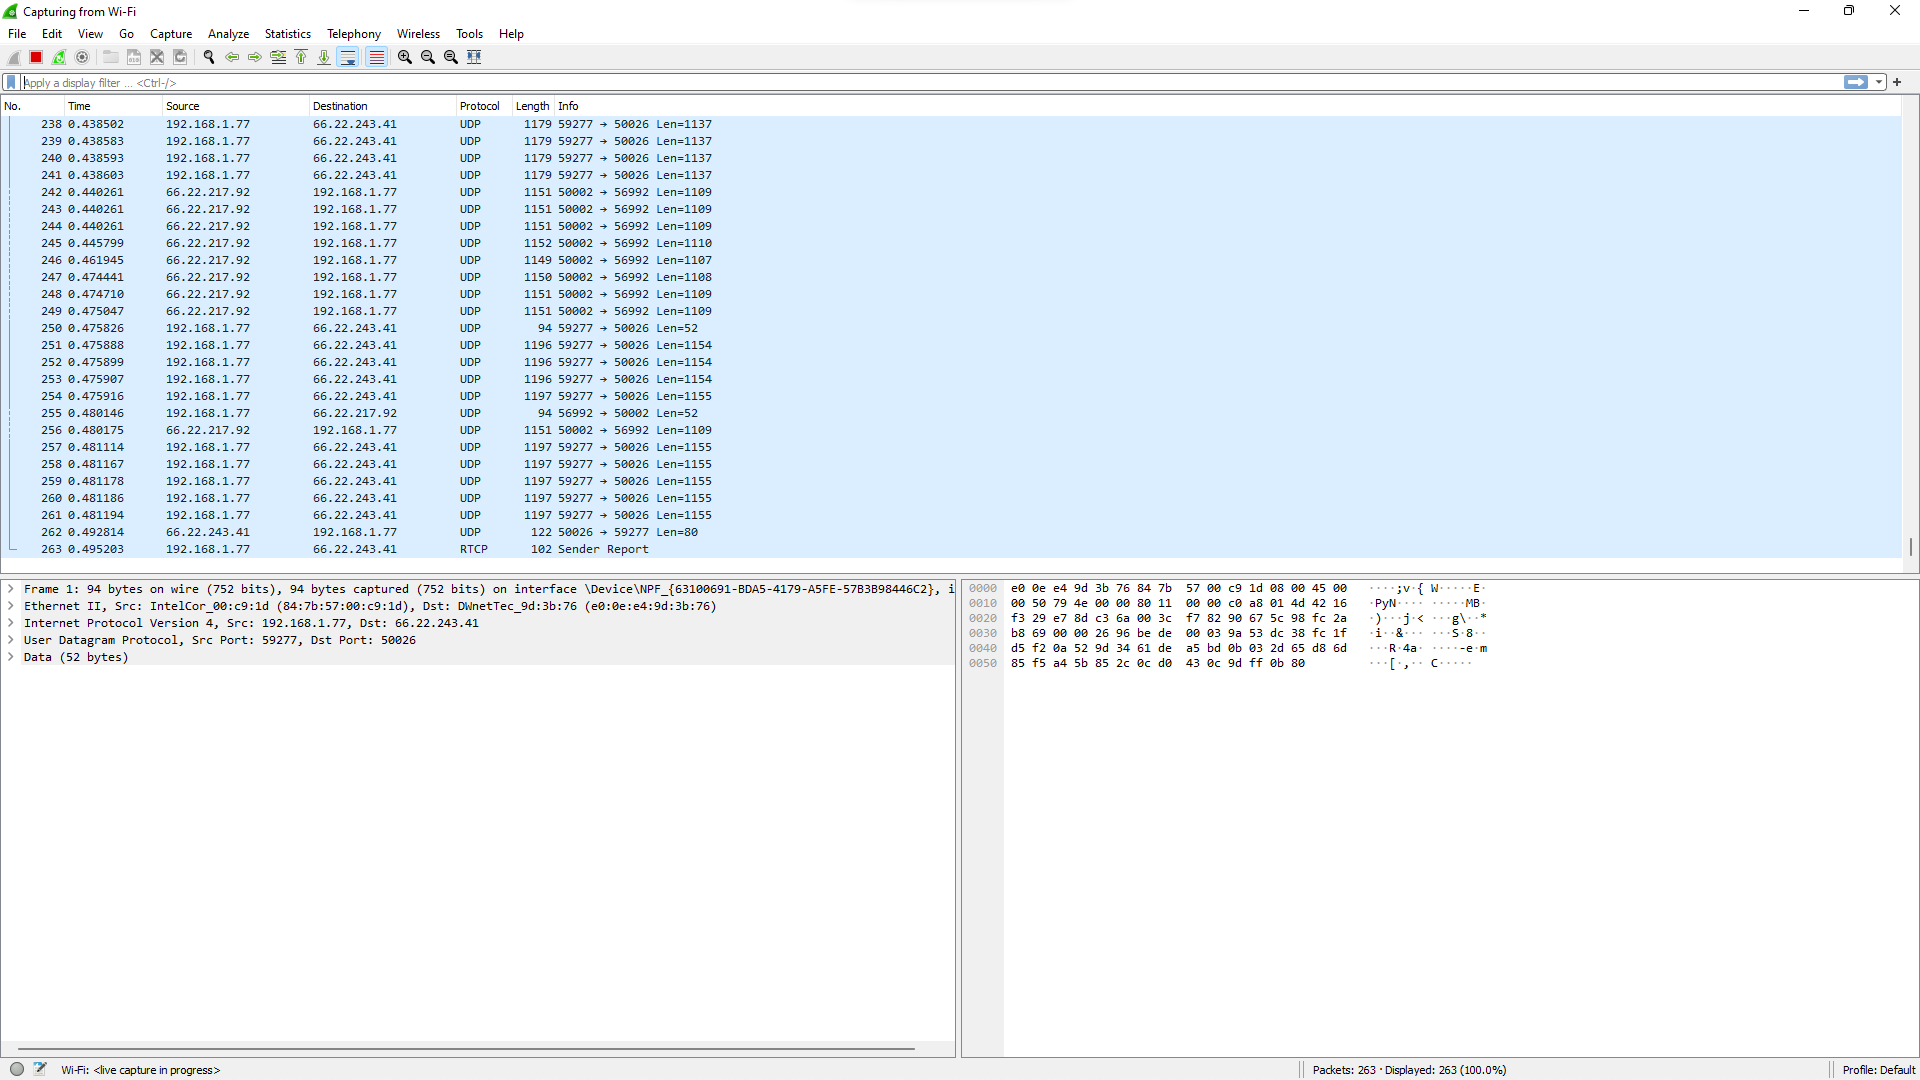
\includegraphics[width=0.85\textwidth]{01_00 (46)}
    \caption{Запущенный захват пакетов}
  \end{figure}

  Далее запустим сканирование хоста с адресом 195.208.245.253
  \begin{figure}[H]
    \centering
    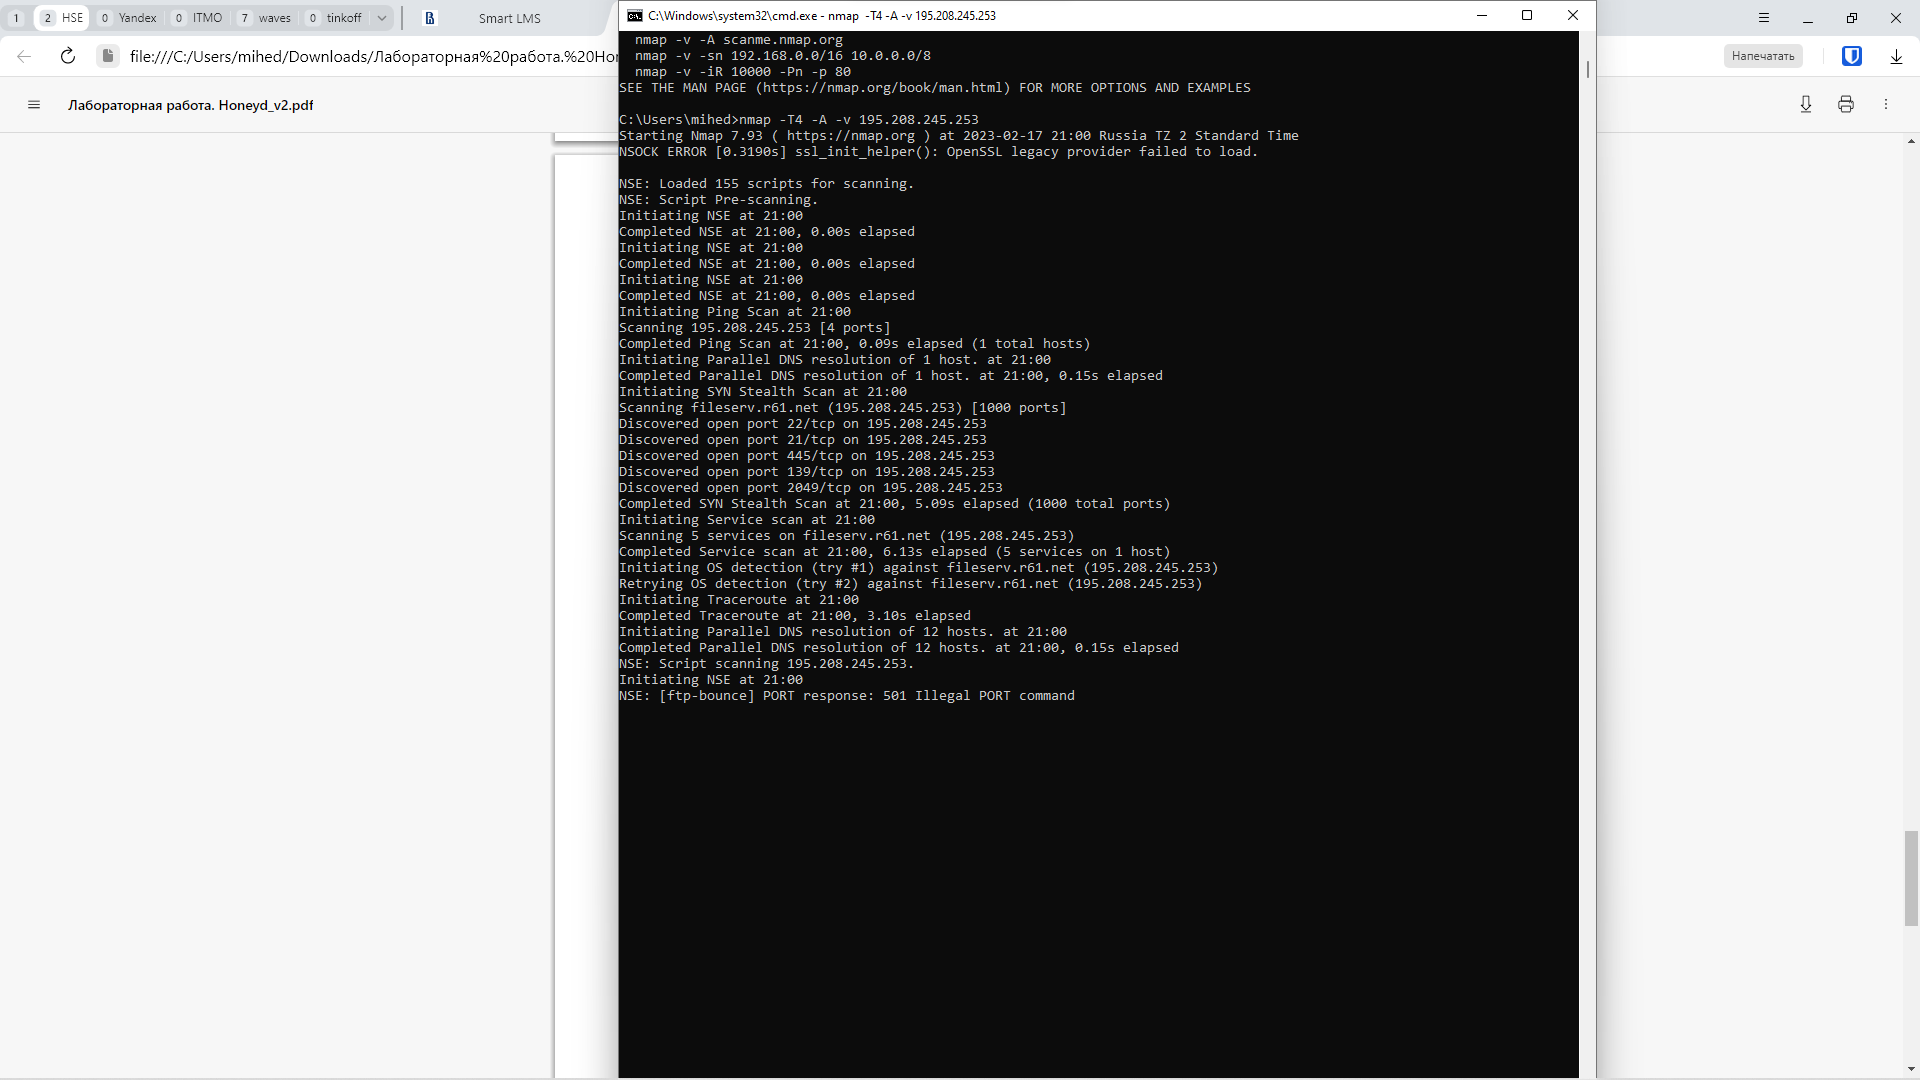
\includegraphics[width=0.85\textwidth]{01_00 (47)}
    \caption{Сканирование портов}
  \end{figure}

  Отфильтруем захваченные пакеты по протоколу \textit{FTP}
  \begin{figure}[H]
    \centering 
    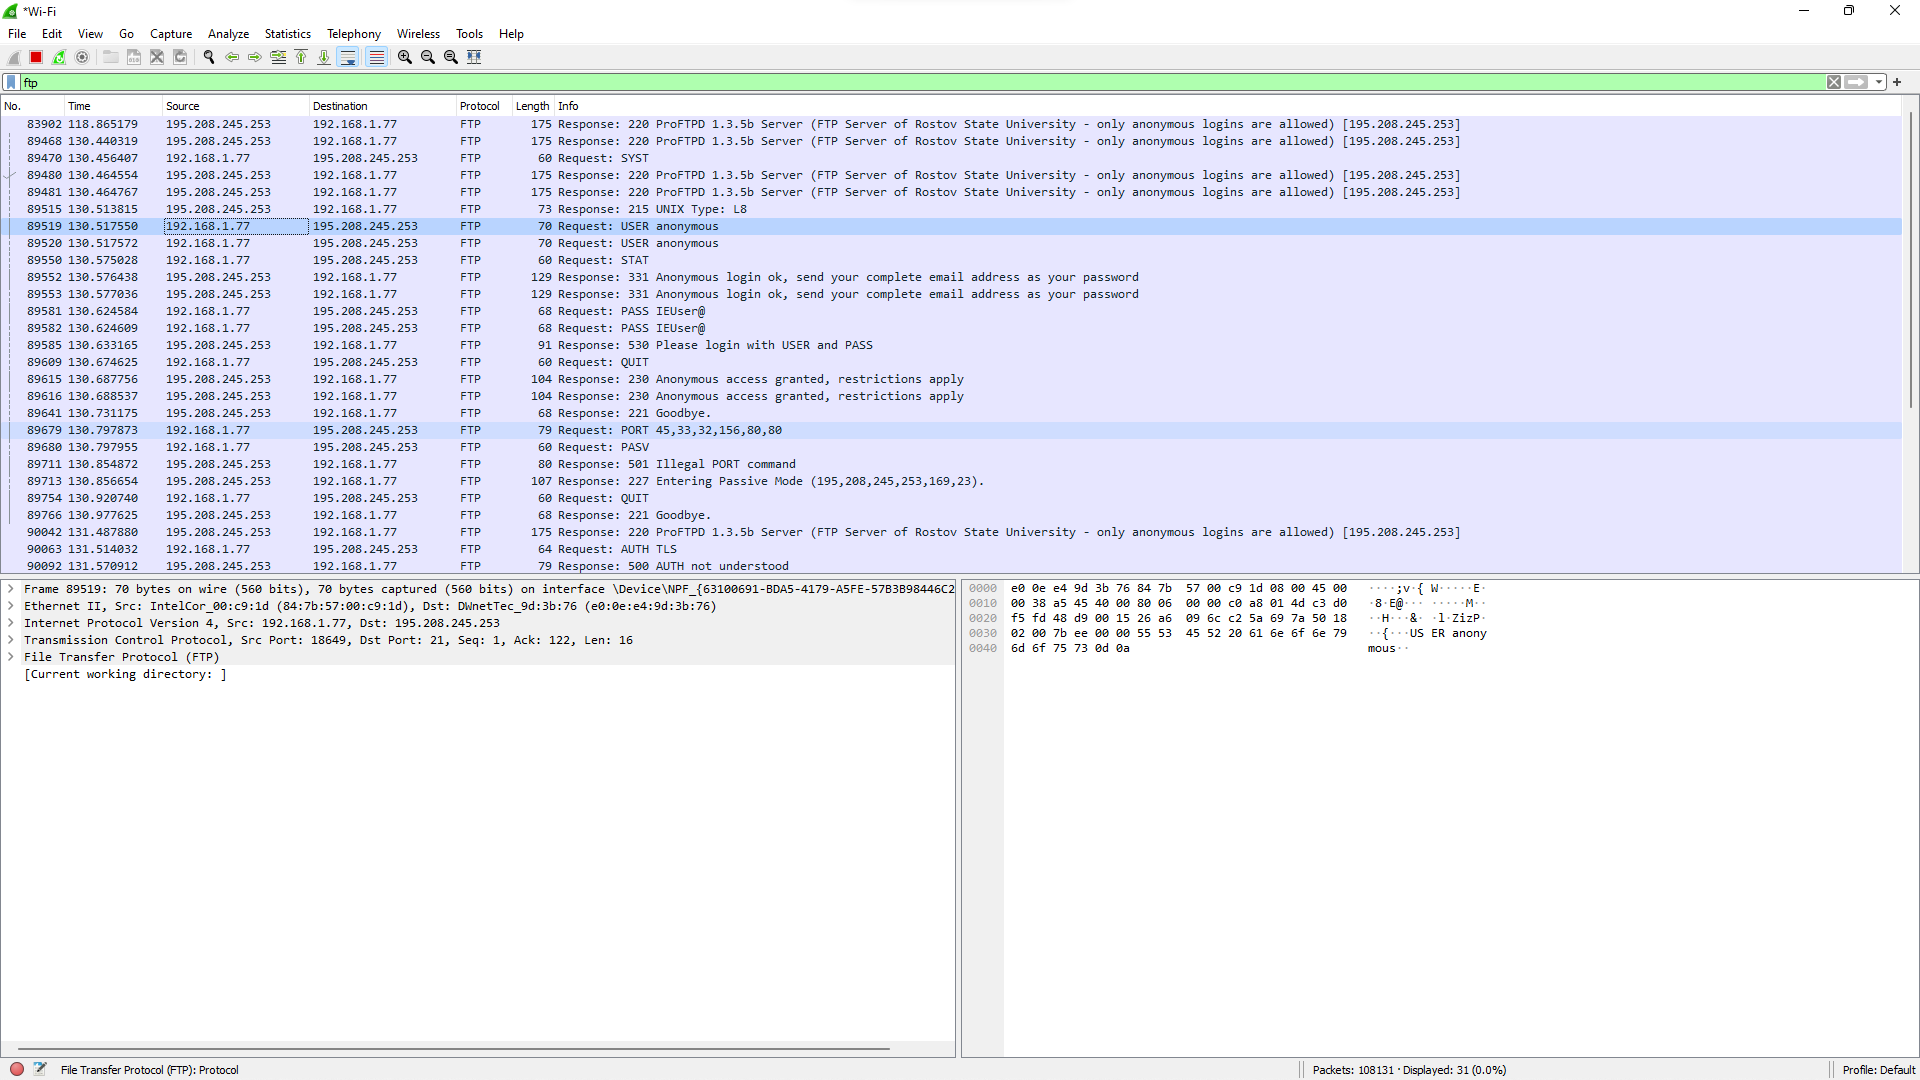
\includegraphics[width=0.85\textwidth]{01_00 (48)}
    \caption{Захваченные FTP пакеты}
  \end{figure}

  Внимательно изучим перехваченные данные, чтобы найти пакет, в котором
  был передан логин пользвателя
  \begin{figure}[H]
    \centering 
    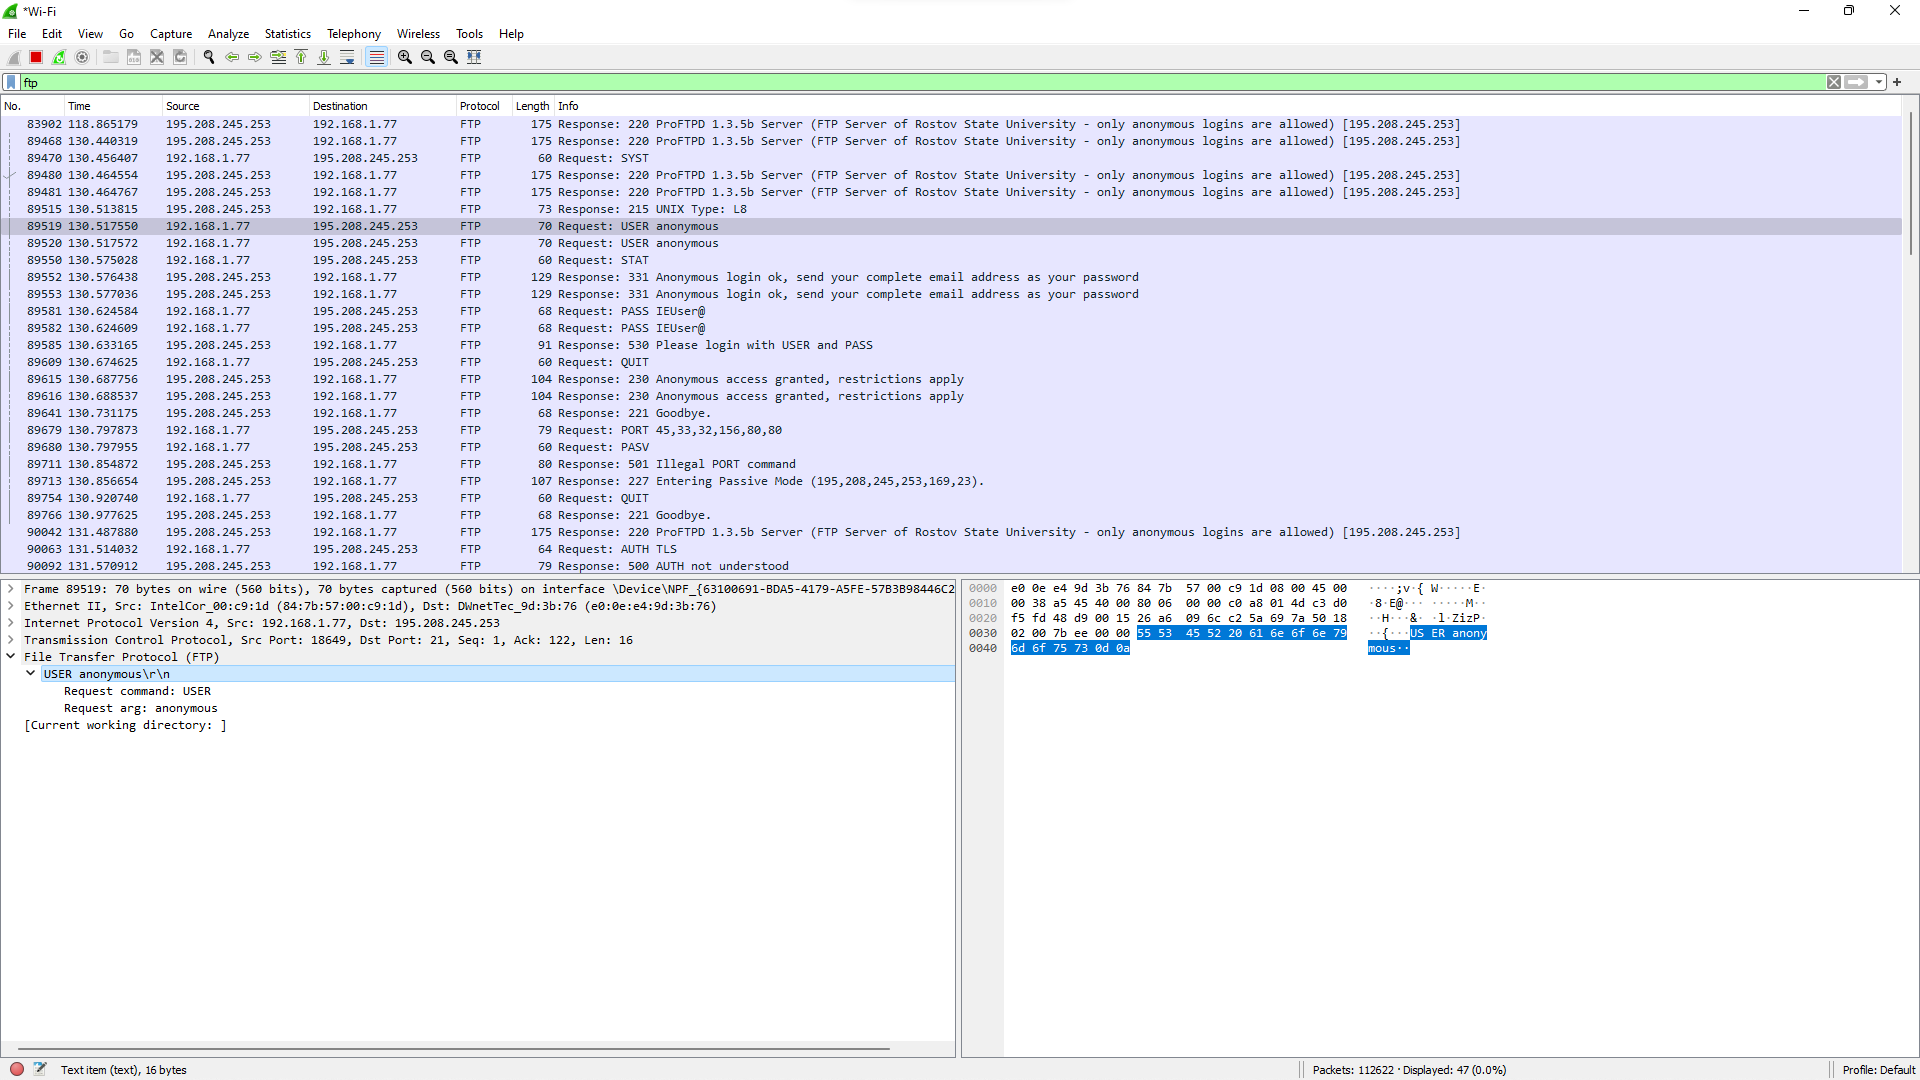
\includegraphics[width=0.85\textwidth]{01_00 (49)}
    \caption{Нужный пакет}
  \end{figure}

  По данному пакету видно, что для авторизации на \textit{FTP} сервере был использован
  логин \textit{anonymous}.

  \section{Вывод}

  В ходе данной лабораторной работы мне удалось научиться работать с виртуальными машинами,
  настраивать связь между ними, в частности при помощи NAT. Также удалось разобраться
  с настройкой и запуском инструмента \textit{honeypot} и научиться сканировать
  порты при помощи \textit{nmap}.

\end{document}

